\documentclass[a4paper,openany,oneside]{book}
\usepackage[utf8]{vietnam}
\usepackage[top=3.5cm, bottom=3cm, left=3.5cm, right=2cm] {geometry}
\usepackage{amssymb,amsthm, makeidx, enumerate, mdframed, pgf,tikz, mathrsfs}
\usetikzlibrary{calc}
\usepackage{scrextend}
\usepackage{fancyhdr}
\usepackage{amsmath}
\usepackage{mathpazo}
\usepackage{hyperref}
\usepackage{url}
\newtheorem{algorithm}{Thuật toán}
\pagestyle{fancy}
\newcommand{\vol}{\textrm{vol}}
\changefontsizes{13pt}
\setlength{\parindent}{0.6cm}
\setlength{\parskip}{0.2cm}
\makeindex
\usepackage{pdfpages}
\usepackage{algorithm}
\makeatletter
\renewcommand{\ALG@name}{Thuật toán}
\makeatother
\usepackage{algpseudocode}
\usepackage{graphicx}
\usepackage{textcomp}
\usepackage{algpseudocode}
% \newtheorem{proof}{Proof}[section]
%\newtheorem{alg}{Thuật toán}[chapter]
\usepackage{multirow}
\usepackage{caption}
\def\BibTeX{{\rm B\kern-.05em{\sc i\kern-.025em b}\kern-.08em
		T\kern-.1667em\lower.7ex\hbox{E}\kern-.125emX}}

\captionsetup[algorithm]{
	labelfont = bf,
	labelsep = period
}

\makeatletter
\newenvironment{breakablealgorithm}
{% \begin{breakablealgorithm}
%		\begin{center}
			\refstepcounter{algorithm}% New algorithm
			~\par
			\hrule height.8pt depth0pt \kern2pt
			\hrule height.8pt depth0pt \kern2pt% \@fs@pre for \@fs@ruled
			\renewcommand{\caption}[2][\relax]{% Make a new \caption
				{\raggedright\textbf{\fname@algorithm~\thealgorithm.} ##2\par}%
				\ifx\relax##1\relax % #1 is \relax
				\addcontentsline{loa}{algorithm}{\protect\numberline{\thealgorithm}##2}%
				\else % #1 is not \relax
				\addcontentsline{loa}{algorithm}{\protect\numberline{\thealgorithm}##1}%
				\fi
%				\kern2pt\hrule\kern1pt
				\vspace{1pt}
				\hrule height.8pt depth0pt \kern2pt
				\hrule height.8pt depth0pt \kern2pt
			}
		}{% \end{breakablealgorithm}
		\kern2pt\hrule\relax% \@fs@post for \@fs@ruled
%	\end{center}
}
\makeatother

\DeclareCaptionFormat{algor}{%
	\hrulefill\par\offinterlineskip\vskip1pt%
	\textbf{#1#2}#3\offinterlineskip\hrulefill}
\DeclareCaptionStyle{algori}{singlelinecheck=off,format=algor,labelsep=space}
\captionsetup[algorithm]{style=algori}

\renewcommand{\listalgorithmname}{Danh sách các thuật toán}
\renewcommand{\listtablename}{Danh sách các bảng}
\renewcommand{\listfigurename}{Danh sách các sơ đồ}
\allowdisplaybreaks
\begin{document}
	\input def
	\pagestyle{myplain}
	\begin{titlepage}
%\thispagestyle{empty}
\begin{center}
{\bf  ĐẠI HỌC QUỐC GIA TP. HỒ CHÍ MINH}\\
{\bf TRƯỜNG ĐẠI HỌC KHOA HỌC TỰ NHIÊN}\\
\hfill

\vspace*{2cm}

{\large\bf  PHAN THÀNH NHÂN}

\vspace*{3cm}

{\LARGE\bf SỬ DỤNG TÍNH TOÁN SONG SONG ĐỂ LỰA CHỌN ĐẶC TRƯNG DỰA TRÊN TIÊU CHÍ TỈ LỆ VẾT	}

\vspace*{3cm}

{\large\bf LUẬN VĂN THẠC SĨ TOÁN HỌC}


\vfill

{\bf TP. Hồ Chí Minh - 2022}
\end{center}
\end{titlepage}


	\newpage
%\thispagestyle{empty}
\begin{center}
{\bf  ĐẠI HỌC QUỐC GIA TP. HỒ CHÍ MINH}\\
{\bf TRƯỜNG ĐẠI HỌC KHOA HỌC TỰ NHIÊN}

\vspace*{1.5cm}

{\bf  PHAN THÀNH NHÂN}

\vspace*{1.5cm}

{\LARGE\bf SỬ DỤNG TÍNH TOÁN SONG SONG ĐỂ LỰA CHỌN ĐẶC TRƯNG DỰA TRÊN TIÊU CHÍ TỈ LỆ VẾT	}

\vspace*{1.5cm}

{\bf LUẬN VĂN THẠC SĨ TOÁN HỌC}\\[20pt]
CHUYÊN NGÀNH CƠ SỞ TOÁN CHO KHOA HỌC DỮ LIỆU\\[10pt]
Mã ngành: 8480109

\vspace*{3cm}

NGƯỜI HƯỚNG DẪN KHOA HỌC

{\bf TS. Nguyễn Thị Thu}

\vfill
\thispagestyle{empty}
{\bf TP. Hồ Chí Minh - 2022}
\end{center}


	\vspace*{3cm}

\begin{center}
	\LARGE{\textbf{Lời cam đoan}}
	\addcontentsline{toc}{chapter}{Lời cam đoan}
\end{center}

Tôi cam đoan luận văn thạc sĩ chuyên ngành Cơ sở Toán cho Khoa học Dữ liệu, với đề tài \lq\lq\textit{Sử dụng tính toán song song để lựa chọn đặc trưng dựa trên tiêu chí tỉ lệ vết}\rq\rq~là công trình khoa học do Tôi thực hiện dưới sự hướng dẫn của TS. Nguyễn Thị Thu và sự hỗ trợ, góp ý của PGS.TS Nguyễn Thanh Bình

Những kết quả nghiên cứu của luận văn hoàn toàn trung thực và chính xác.

\begin{flushright}
	Học viên cao học\hskip 2cm\quad
	
	\vskip 2cm
	
	{Phan Thành Nhân} \hskip 1.5cm\quad\
\end{flushright}
\thispagestyle{empty}
	\vspace*{3cm}

\begin{center}
\LARGE{\textbf{Lời cảm ơn}}
\end{center}


Lời đầu tiên, tôi xin gửi lời cảm ơn chân thành tới TS. Nguyễn Thị Thu, người vừa là người thầy, vừa là người chị đã giúp đỡ tôi rất nhiều, người đã từng bước định hướng và trang bị cho tôi những kiến thức cần thiết, hướng dẫn và chỉ bảo tận tình cho tôi trong suốt quá trình học tập, nghiên cứu cũng như thực hiện luận văn này. Tôi cũng xin gửi lời cảm ơn đến PGS. TS. Nguyễn Thanh Bình, người đã tạo điều kiện và hỗ trợ tôi rất nhiều, thầy thường chia sẻ và cho tôi rất nhiều lời khuyên và góp ý trong việc định hướng nghiên cứu trong suốt thời gian tôi theo học chương trình thạc sĩ ở khoa Toán. Trong quá trình thực hiện luận văn này, tôi đã gặp không ít khó khăn do thời gian không nhiều cũng như kiến thức còn hạn chế, tuy nhiên tôi luôn nhận được sự quan tâm, giúp đỡ, động viên đến từ gia đình, thầy cô, bạn bè.

Tôi xin chân thành cảm ơn đến các thầy cô trong khoa Toán và các thầy cô được mời giảng dạy trong chương trình thạc sĩ này, các thầy cô đã trực tiếp trang bị cho tôi kiến thức toán cũng như phương pháp tự học, tự nghiên cứu. Lời cuối cùng, để hoàn thành luận văn, tôi đã sử dụng, tham khảo một số tài liệu và bài viết, xin cảm ơn các tác giả.

\begin{flushright}
{\it TP.HCM, \today}

Tác giả\hskip 2.5cm\quad

\vskip 1cm

{\bf Phan Thành Nhân} \hskip 1cm \quad\ 
 \end{flushright}
\thispagestyle{empty}

	\thispagestyle{empty}
\begin{center}
	\LARGE{\textbf{TRANG THÔNG TIN LUẬN VĂN}}
	\addcontentsline{toc}{chapter}{Trang thông tin luận văn tiếng Việt}
\end{center}

\noindent Tên đề tài luận văn: Sử dụng tính toán song song để lựa chọn đặc trưng dựa trên tiêu chí tỉ lệ vết
\\
Ngành: Cơ sở Toán cho Khoa học Dữ liệu
\\
Mã số ngành: 8480109
\\
Họ tên học viên cao học: Phan Thành Nhân
\\
Khóa đào tạo: 2020 - 2022
\\
Người hướng dẫn khoa học: TS. Nguyễn Thị Thu.
\\
Cơ sở đào tạo: Trường Đại học Khoa học Tự nhiên, ĐHQG.HCM\\
\\
{\bf 1. TÓM TẮT NỘI DUNG LUẬN VĂN:}
\begin{itemize}
	\item[-] Chương 1: Giới thiệu tổng quan về lựa chọn đặc trưng và các nghiên cứu liên quan.
	\item[-] Chương 2: Trình bày về tiêu chí vết - tiếu chí lựa chọn đặc trưng. Sau đó chứng minh các kết quả và cuối cùng trình bày Thuật toán PSFT - thuật toán lựa chọn đặc trưng song song dựa trên tiêu chí vết.
	\item[-] Chương 3: Trình bày về các tập dữ liệu được sử dụng khi làm thực nghiệm. Thông tin về phần cứng được sử dụng và thảo luận kết quả thực nghiệm.
 	\item[-] Cuối cùng: Phần kết luận và danh mục các tài liệu tham khảo.
	
\end{itemize}

\noindent {\bf 2. NHỮNG KẾT QUẢ MỚI CỦA LUẬN VĂN:} 

Xây dựng một thuật toán lựa chọn đặc trưng song song dựa trên tiêu chí vết (thuật toán PFST) trên các tập dữ liệu lớn. Thuật toán sử dụng tiêu chí vết để đánh giá các đặc trưng tốt. Thực nghiệm cho thấy thuật toán cho kết quả tốt không chỉ về mặt hiệu suất của mô hình LDA cho bài toán phân loại mà còn tiết kiệm chi phí tính toán, khi thời gian chạy và đạt kết quả nhanh chóng.

\noindent {\bf 3. CÁC ỨNG DỤNG/ KHẢ NĂNG ỨNG DỤNG TRONG THỰC TIỄN HAY NHỮNG VẤN ĐỀ CÒN BỎ NGỎ CẦN TIẾP TỤC NGHIÊN CỨU:}
Kết quả luận văn có thể được dùng để lựa chọn đặc trưng trên các tập dữ liệu thực tế. Tuy nhiên, một trong những nhược điểm của PFST là tiêu chí vết chỉ có thể sử dụng cho các đặc trưng liên tục. Do đó, trong tương lại, chúng tôi vẫn sẽ nỗ lực làm việc, và hi vọng sẽ khám phá ra cách mở rộng cho các trường hợp còn lại trong bài toán phân loại.
\newpage

\begin{tabular}{ccccc}
 {\bf CÁN BỘ HƯỚNG DẪN}	&&&& {\bf HỌC VIÊN CAO HỌC} \\
 (Ký tên, họ tên) &&&& (Ký tên, họ tên) \\
\end{tabular}

\vspace{3cm}

\begin{center}
{\bf XÁC NHẬN CỦA CƠ SỞ ĐÀO TẠO}

{\bf HIỆU TRƯỞNG}
\end{center}
\thispagestyle{empty}
	\thispagestyle{empty}
\begin{center}
	\LARGE{\textbf{THESIS INFORMATION}}
	\addcontentsline{toc}{chapter}{Trang thông tin luận văn tiếng Anh}
\end{center}

\noindent Thesis title: Parallel feature selection based on the trace ratio criterion
\\
Speciality: Data science
\\
Code:  8480109
\\
Name of Master Student: Phan Thành Nhân
\\
Academic year: 2020 - 2022
\\
Supervisor:  Dr. Nguyen Thi Thu
\\
At: VNUHCM - University of Science\\
\\
{\bf 1. SUMMARY:}
\begin{itemize}
	\item[-] Chapter 1: An overview of feature selection and related works.
	\item[-] Chapter 2: Present trace criterion as a feature selection criterion. Prove the results and present parallel Feature Selection  using  Trace  criterion (PFST Algorithm).
	\item[-] Chapter 3: Presentation of the experiment's data sets. Discussion of the experimental findings and information on the hardware utilized.
        \item[-] Finally: Conclusion and list of references.
\end{itemize}

\noindent {\bf 2. NOVELTY OF THESIS:}  The main results in this thesis are as follows. 

Presents a novel parallel feature selection approach for classification, called PFST, for feature selection on large-scale datasets. The method uses the trace criterion. The experiments show that our PFST method achieves good accuracy using the LDA model and less running time to select relevant features.

\noindent {\bf 3. APPLICATIONS/ APPLICABILITY/ PERSPECTIVE:}

The results of this thesis can be used to select the features of the real data sets. However, one of the drawbacks of the algorithm is that the trace criterion can only be used for continuous features. Therefore, in the future, it would be desirable to explore how to extend this work to the case where there are categorical features in the model as well.
\newpage

\begin{center}
\begin{tabular}{ccccccccccccc}
	{\bf SUPERVISOR}	&&&&&&&&&&&& {\bf Master STUDENT} \\
\end{tabular}
\end{center}

\vspace{3cm}

\begin{center}
	{\bf CERTIFICATION}\\ 
	{\bf UNIVERSITY OF SCIENCE}\\
	{\bf PRESIDENT}
\end{center}
\thispagestyle{empty}
	\tableofcontents
	\listoffigures
	\listoftables
	\listofalgorithms
	\chapter*{Lời nói đầu}
\addcontentsline{toc}{chapter}{Lời nói đầu}

Sự phát triển của dữ liệu ngày nay đặt ra thách thức trong quản lý, lưu trữ và áp dụng vào các bài toán cụ thể. Trong khi các phương pháp trích xuất đặc trưng có thể giảm kích thước dữ liệu để thực hành, nhưng các phương pháp này không giúp giảm thiểu chi phí lưu trữ dữ liệu. Trong khi đó, việc lựa chọn đặc trưng giúp loại bỏ các đặc trưng dư thừa và do đó hữu ích không chỉ trong thực hành nghiên cứu dữ liệu mà còn trong giảm chi phí quản lý và lưu trữ.  Trong đề tài luận văn cao học này, chúng tôi phát triển một phương pháp \lq\lq Sử dụng tính toán song song để lựa chọn đặc trưng dựa trên tiêu chí tỉ lệ vết (Parallel feature selection based on the trace ratio criterion - PFST)\rq\rq cho bài toán phân loại. Tiêu chí được sử dụng là một thước đo về khả năng tách lớp được sử dụng trong LDA, để đánh giá tính hữu dụng của đặc trưng. Dựa trên tiêu chí này, PFST sẽ nhanh chóng tìm thấy các đặc trưng quan trọng từ một tập hợp các đặc trưng gốc của tập dữ liệu lớn bằng cách sử dụng sức mạnh của tính toán song song để thực hiện lựa chọn đặc trưng và loại bỏ các đặc trưng dư thừa. Sau khi các đặc trưng quan trọng nhất được đưa vào mô hình, chúng tôi đánh giá phương pháp thông qua các thử nghiệm khác nhau bằng cách sử dụng LDA làm mô hình phân loại. Thực nghiệm cho thấy rằng phương pháp của chúng tôi có thể chọn ra một tập hợp con nhỏ các đặc trưng trong thời gian ngắn, tiết kiệm thời gian hơn so với một số phương pháp khác. Ngoài ra, độ chính xác khi phân loại dựa trên các đặc trưng được lựa chọn bằng PFST cũng đạt độ chính xác cao và tốt hơn các phương pháp khác, và tốt hơn việc phân loại dựa trên tập các đặc trưng gốc ban đầu.

Nội dung khóa luận này bao gồm 4 chương. Trong đó,
\begin{description}
	\item[Chương 1:] Chương này giới thiệu tổng quan về lý do chọn đề tài và các nghiên cứu khoa học liên quan.
	\item[Chương 2:] Chương này trình bày các kiến thức nền tảng về vấn đề lựa chọn đặc trưng cho lớp các bài toán phân loại.
	\item[Chương 3:] Chương này trình bày về tiêu chí vết - tiếu chí lựa chọn đặc trưng. Thuật toán PSFT - thuật toán lựa chọn đặc trưng song song dựa trên tiêu chí vết.
	\item[Chương 4:] Chương này trình bày về các tập dữ liệu được sử dụng khi làm thực nghiệm và thông tin về phần cứng được sử dụng. Trình bày các thuật toán được dùng để so sánh với PFST và thảo luận kết quả
	\item[Cuối cùng:] Phần kết luận và danh mục các tài liệu tham khảo.
\end{description}

	\chapter{Tổng quan}\label{chapter:tq}

\section{Lý do chọn đề tài}
Trong kỷ nguyên của dữ liệu lớn, sự phát triển của dữ liệu đặt ra những thách thức đối với việc quản lý và sử dụng dữ liệu hiệu quả. Ví dụ: một tập dữ liệu gen có thể chứa hàng trăm nghìn đặc điểm \cite{guyon2007competitive}. Do đó, việc xử lý trực tiếp các tập dữ liệu như vậy có thể gặp sự khó khăn về kích thước. Hơn nữa, các đặc trưng dư thừa có thể làm giảm hiệu suất học tập của các thuật toán phân loại. Để giải quyết vấn đề này, nhiều kỹ thuật giảm chiều dữ liệu đã được phát triển \cite{melab2006grid,de2006parallelizing,garcia2006parallel,guillen2009efficient,lopez2006solving} và chúng được phân loại thành các phương pháp trích xuất đặc trưng hoặc lựa chọn đặc trưng \cite{liu2012feature, kumar2014feature}. Kỹ thuật trích xuất đặc trưng (ví dụ: Phân tích thành phần chính (Principal Component Analysis - PCA) \cite{johnson2002applied}, Phân tích phân biệt tuyến tính (Linear Discriminant Analysis - LDA) \cite{johnson2002applied}) liên quan đến việc chiếu dữ liệu vào một không gian đối tượng mới với số chiều nhỏ hơn thông qua một vài bước biến đổi tuyến tính hoặc phi tuyến từ các đặc trưng gốc. Tuy nhiên, điều này tạo ra một loạt các đặc trưng mới mà không thể diễn giải trực tiếp. Hơn nữa, vì những cách tiếp cận đó sử dụng tất cả các đặc trưng có sẵn trong quá trình trích xuất đặc trưng nên nó không giúp giảm chi phí lưu trữ dữ liệu và chi phí thu thập dữ liệu trong tương lai. Mặt khác, các phương pháp lựa chọn đặc trưng (\cite{sinaga2021entropy, james2013introduction},\ldots) chỉ chọn một tập hợp con các đặc trưng hữu ích để xây dựng mô hình. Do đó, điều này giúp giữ các tính chất của các đặc trưng ban đầu trong khi giảm chi phí lưu trữ và thu thập dữ liệu trong tương lai bằng cách loại bỏ các đặc trưng không liên quan. Tuy nhiên, các dữ liệu từ các lĩnh vực khác nhau như khai thác văn bản, phân tích kinh doanh và sinh học, thường được đo bằng gigabyte hoặc terabyte với hàng triệu đặc trưng \cite{bolon2015feature, li2017feature}. Ví dụ: tập dữ liệu Amazon Review \cite{ni2019justifying} là tập dữ liệu 34 gigabyte. Trong những trường hợp như vậy, hiệu suất của các kỹ thuật lựa chọn đặc trưng mới nhất có thể bị ảnh hưởng  \cite{li2017feature}. Điều này là do không gian tìm kiếm cho một tập hợp con các đặc trưng hữu ích bị tăng lên đáng kể. Một cách để giải quyết vấn đề này là sử dụng tính toán song song, cho phép sử dụng tốt hơn tài nguyên tính toán của máy tính bằng cách phân vùng dữ liệu và chạy các lựa chọn đặc trưng trên nhiều lõi cùng một lúc.

Từ những lý do trên, trong đề tài luận văn cao học này, chúng tôi nghiên cứu và trình bày một phương pháp \lq\lq Sử dụng tính toán song song để lựa chọn đặc trưng dựa trên tiêu chí tỉ lệ vết (Parallel feature selection based on the trace ratio criterion - PFST)\rq\rq cho bài toán phân loại. Tiêu chí đánh giá mức độ hữu dụng của đặc trưng được sử dụng là một thước đo về khả năng tách lớp được sử dụng trong bài toán Linear discriminant analysis (LDA - chúng tôi sẽ trình bày bài toán này bên dưới). Dựa trên tiêu chí này, PFST sẽ nhanh chóng tìm thấy các đặc trưng quan trọng từ một tập hợp các đặc trưng gốc của tập dữ liệu lớn và loại bỏ các đặc trưng dư thừa. Bên cạnh đó, chúng tôi thiết lập và sử dụng tính toán song song để tối ưu nguồn tài nguyên của máy tính nhằm tăng hiệu suất tính toán và thời gian chạy. Cuối cùng, chúng tôi sẽ sử dụng LDA làm mô hình phân loại để đánh giá độ hiệu quả của thuật toán PFST. Bên cạnh đó, chúng tôi cũng so sánh với một số thuật toán khác. Kết quả thu được rất tốt, PFST có thời gian chạy và có độ chính xác cao hơn các phương pháp khác. Bên cạnh đó, tập đặc trưng thu được từ PFST cũng cho ra kết quả tốt hơn nếu sử dụng toàn bộ đặc trưng ban đầu.

\section{Các công trình nghiên cứu khoa học có liên quan}\label{section:relative_work}
Đối mặt với các thách thức về kích thước của dữ liệu ngày càng tăng, đã có nhiều nỗ lực trong hướng nghiên cứu về lựa chọn đặc trưng để phát triển các kỹ thuật mới. Bên cạnh các phương pháp lai để kết hợp các chiến lược lựa chọn đặc trưng khác nhau \cite{saeys2007review,ang2015supervised}, hầu hết các phương pháp lựa chọn đặc trưng có thể được chia thành ba loại.

Đầu tiên, cách tiếp cận \lq\lq wrapper\rq\rq~ dựa trên hiệu suât của một thuật toán học máy cụ thể để đánh giá tầm quan trọng của các đặc trưng được chọn. Một phương pháp \lq\lq wrapper\rq\rq~ điển hình sẽ tìm kiếm một tập con các đặc trưng dựa trên một thuật toán học máy trước, sau đó sẽ đánh giá chúng. Các bước này được lặp lại cho đến khi thỏa mãn một số tiêu chí dừng. Các phương pháp trong loại này thường rất tốn kém về chi phí tính toán vì việc đánh giá tập con các đặc trưng yêu cầu nhiều lần lặp lại. Mặc dùng nhiều các tiếp cận tìm kiếm được đề xuất chẳng hạn như thuật toán tìm kiếm best-first \cite{arai2016unsupervised} và thuật toán di chuyền (genetic) \cite{goldberg1988genetic}. Tuy nhiên, việc sử dụng các thuật toán này cho dữ liệu nhiều chiều vẫn không cho thấy sử cải thiện về chi phí tính toán.

Thứ hai, cách tiếp cận \lq\lq filter\rq\rq~ bao gồm các kỹ thuật đánh giá các tập hợp con đặc bằng việc xếp hạng với một số tiêu chí như tiêu chí thông tin \cite{nguyen2014effective, shishkin2016efficient}, khả năng tái tạo \cite{farahat2011efficient, masaeli2010convex}. Các phương pháp này chọn các đặc trưng độc lập với thuật toán học máy và thường hiệu quả hơn về chi phí tính toán so với các phương pháp \lq\lq wrapper\rq\rq~\cite{li2017feature}. Tuy nhiên, vì không được tối ưu hóa cho bất kỳ thuật toán học máy mục tiêu nào, nên chúng có thể không tối ưu cho một tuật toán học máy cụ thể.

Thứ ba, các phương pháp \lq\lq embedded\rq\rq~ sử dụng các tiêu chí độc lập để tìm ra tập con tối ưu cho một tập hợp nhất định. Sau đó, một thuật toán học máy được sử dụng để lựa chọn tập con tối ưu cuối cùng trong số các tập con tối ưu trên các tập hợp khác nhau. Vì thế, chúng hiệu quả hơn về chi phí tính toán so với các phương pháp \lq\lq wrapper\rq\rq~ vì chúng không đánh giá đặc trưng dựa trên việc lặp lại các tập con đặc trưng. Ngoài ra, chúng cũng được huấn luyện từ các thuật toán học máy. Vì thế, chúng có thể được coi như sự đánh đổi giữa phương pháp \lq\lq filter\rq\rq~ và phương pháp \lq\lq wrapper\rq\rq \cite{li2017feature}.

Mặc dù, cho đến này, các nhà khoa học đã nỗ lực rất nhiều trong hướng nghiên cứu lựa chọn đặc trưng, nhưng dữ liệu từ các trường, các ngành khác nhau có thể quá phong phú ngay cả đối với các phương pháp \lq\lq filter\rq\rq hiệu quả về chi phí tính toán. Điều này đã thúc đẩy nhiều nghiên cứu khác trong việc lựa chọn đặc trưng song song. Một số phương pháp đã được đề xuất trong \cite{melab2006grid,de2006parallelizing,garcia2006parallel,guillen2009efficient,lopez2006solving} sử dụng quy trình xử lý song song để đánh giá đồng thời nhiều đặc trưng. Tuy nhiên, các thuật toán này yêu cầu quyên truy cập vào toàn bộ dữ liệu. Mặc khác, trong trong \cite{singh2009parallel}, các tác giả đã đề xuất một thuật toán lựa chọn đặc trưng song song cho hồi quy logistic dựa trên framework MapReduce và các đặc trưng được đánh giá thông qua hàm mục tiêu của mô hình hồi quy logistic. Trong khi đó, các tác giả của bài báo \cite{tsamardinos2019greedy} đã đề xuất \textit{Song song, Tiến–Lùi với thuật toán Tỉa (Parallel, Forward–Backward with Pruning algorithm)} (PFBP) để lựa chọn đặc trưng bằng cách bỏ sớm một số đặc trưng trong các lần lặp lại tiếp theo và sớm trả ra kết quả đặc trưng tốt nhất trong mỗi lần lặp. Tuy nhiên, các tiếp cận này yêu cầu tính toán bootstrap của p-giá trị, rất tốn kém chi phí tính toán. Trong bài báo \cite{zhao2013massively}, Zhao và các cộng sự đã giới thiệu một thuật toán lựa chọn đặc trưng song song để chọn các đặc trưng dựa trên khả năng giải thích phương sai của dữ liệu. Tuy nhiên, theo các tiếp cận của họ, việc xác định số lượng các đặc trưng trong mô hình dựa trên việc chuyển đổi các nhãn phân loại thành các giá trị số và sử dụng tổng bình phương sai số. Việc tính tổng bình phương sai số đòi hỏi phải điều chỉnh mô hình và do đó thuật toán vẫn còn tốn kém rất nhiều chi phí tính toán.
	\chapter{Kiến thức nền tảng}

\section{Quy trình của lớp các bài toán phân loại}
Để giải quyết một bài toán phân loại, ta cần phải hiểu dữ liệu, tính chất các đặc trưng và quá trình chọn các đặc trưng phù hợp với mô hình cũng cần phải có một quy trình rõ ràng.

Bước đầu tiên là xác định bài toán, nghĩa là xác định nhãn của bài toán và xây dựng tập dữ liệu (data collection). Phải đảm bảo là tập dữ liệu phải liên quan đến bài toán được mô hình hóa. Bước này rất quan trọng vì sẽ ảnh hưởng rất nhiều đến kết quả phân loại. Ngoài ra, chỉ những đặc trưng có thông tin hữu ích về bài toán là nên được sử dụng. Trong một số trường hợp, khi gặp khó khăn về kiến thức cũng như khả năng thu thập dữ liệu. Chúng ta có thể sử dụng phương pháp brute-force để thay thế. Brute-force là một phương pháp giải quyết vấn đề bằng cách thực hiện tất cả các giải pháp có thể có và chọn ra giải pháp tốt nhất. Nó được sử dụng khi không có một thuật toán cụ thể nào có thể giải quyết vấn đề hoặc khi không có đủ kiến thức về vấn đề để thiết kế một giải pháp tối ưu. Tuy nhiên, phương pháp này có thể rất tốn kém và thời gian, đặc biệt là đối với các vấn đề có kích thước lớn. Do vậy, trong trường hợp này sẽ có một lượng rất lớn các biến được đo, xử lý và thêm vào tập dữ liệu. Tuy nhiên, hi vọng, trong tương lại có thể tác được các đặc trưng tốt nhất và phù hợp nhất với bài toán.

Nếu vấn đề về dữ liệu có thể được giải quyết, chúng ta sẽ nên bước tiếp theo trong quy trình phân loại là tiền xử lý dữ liệu (data pre-processing). Ở bước này, vấn đề chính là thiếu dữ liệu (missing data) và dữ liệu ngoại lai (outlier) cần phải được xử lý. Có một vài phương pháp phân tích thống kê \cite{aggarwal2001outlier, hodge2004survey} để có thể dử lý các vấn đề này. Hơn nữa, đây là bước mà số lượng các đặc trưng của bài toán có thể giảm đi bằng việc áp dụng thuật toán lựa chọn đặc trưng.

Vấn đề này có thể được giải quyết, đưa chúng ta đến bước tiếp theo trong quy trình phân loại: tiền xử lý dữ liệu. Ở giai đoạn này, các vấn đề chính như giá trị bị thiếu và phát hiện ngoại lệ nên được xử lý. Có nhiều phương pháp phân tích thống kê để giải quyết các vấn đề này [1, 26]. Ngoài ra, đây là giai đoạn trong vấn đề mà số lượng đặc trưng của vấn đề có thể được giảm bằng thuật toán lựa chọn đặc trưng.

Bước tiếp theo là lựa chọn thuật toán phân loại. Có rất nhiều các thuật tóa phân loại, và mặc dù các thuật toán rất đa dạng và khác nhau về ý tưởng, nhưng không dễ dàng chọn được thuật toán nào là tốt nhất cho một bài toán cụ thể. Do đó, việc thử nghiệm và so sánh một số thuật toán là một cách làm tương đối phổ biến, mục tiêu cuối cùng là lựa chọn được thuật toán cho kết quả tốt nhất \cite{kotsiantis2007supervised}.

Việc đánh giá các thuật toán phân loại thường dựa trên độ chính xác của việc dự đoán. Một kỹ thuật điển hình là chia dữ liệu thành hai phần để huấn luyện mô hình và sử dụng phần còn lại để kiểm tra độ chính xác. Tuy nhiên, quy trình này thường dẫn đến kết quả không tốt khi áp dụng vào tập dữ liệu bên ngoài. Do đó, để giảm thiểu sai số, một số kỹ thuật phức tạp hơn như kiểm tra chéo (cross-validation) \cite{kohavi1995study} có thể được sử dụng.

Để có cái nhìn tổng quan, chúng tôi xin trình bày theo sơ đồ khối của toàn bộ quy trình của một bài toán phân loại.

\begin{figure}
	\centering
	\begin{tikzpicture}[thick, scale=0.8, every node/.style={scale=0.7}]
		\path
		(0:0) coordinate (O)
		(0:3) coordinate (A)
		(0:6.5) coordinate (B)
		(0:10) coordinate (C)
		(0:13.5) coordinate (D)
		(0:17) coordinate (E)
		(D) ++ (-90:3) coordinate (F)
		(E) ++ (-90:5) coordinate (G)
		(G) ++ (-90:3) coordinate (H)
		;
		\draw 
		(O) circle (1)
		($(A)+(180:1.25)+(-90:0.5)$) rectangle ($(A)+(0:1.25)+(90:0.5)$)
		($(B)+(180:1.25)+(-90:0.5)$) rectangle ($(B)+(0:1.25)+(90:0.5)$)
		($(C)+(180:1.25)+(-90:1)$) rectangle ($(C)+(0:1.25)+(90:1)$)
		($(D)+(180:1.25)+(-90:0.5)$) rectangle ($(D)+(0:1.25)+(90:0.5)$)
		($(E)+(180:1.25)+(-90:0.5)$) rectangle ($(E)+(0:1.25)+(90:0.5)$)
		
		($(F)+(180:1.25)+(-90:0.5)$) rectangle ($(F)+(0:1.25)+(90:0.5)$)
		
		(G)+(180:1)--+(90:1)--+(0:1)--+(-90:1)--cycle
		
		($(H)+(180:1.25)+(-90:0.5)$) rectangle ($(H)+(0:1.25)+(90:0.5)$)
		;
		\path 
		(O) ++ (90:0.25) node{Xác định} ++ (-90:0.5) node{bài toán}
		
		(A) ++ (90:0.25) node{Xây dựng} ++ (-90:0.5) node{tập dữ liệu}
		
		(B) ++ (90:0.25) node{Tiền xử lý} ++ (-90:0.5) node{dữ liệu}
		
		(C) ++ (90:0.5) node{Lựa chọn} ++ (-90:0.5) node{mô hình} ++ (-90:0.5) node{phân loại}
		
		(D) ++ (90:0.25) node{Huấn luyện} ++ (-90:0.5) node{mô hình}
		
		(E) ++ (90:0.25) node{Đánh giá} ++ (-90:0.5) node{mô hình}
		
		(F) ++ (90:0.25) node{Điều chỉnh} ++ (-90:0.5) node{tham số}
		(G) ++ (90:0.25)node {Kiểm} ++ (-90:0.5)node{tra}
		(H) node {Kết thúc}
		;
		\draw[->]
		($(O) + (0:1)$) -- ($(A)+(180:1.25)$)
		;
		
		\draw[->] ($(A) + (0:1.25)$) -- ($(B)+(180:1.25)$);
		\draw[->] ($(A) + (-90:5)$) -- ($(A)+(-90:0.5)$);
		
		\draw[->] ($(B) + (0:1.25)$) -- ($(C)+(180:1.25)$);
		\draw[->] ($(B) + (-90:5)$) -- ($(B)+(-90:0.5)$);
		
		\draw[->] ($(C) + (0:1.25)$) -- ($(D)+(180:1.25)$);
		\draw[->] ($(C) + (-90:5)$) -- ($(C)+(-90:1)$);
		
		\draw[->] ($(D) + (0:1.25)$) -- ($(E)+(180:1.25)$);
		\draw[->] ($(D) + (-90:5)$) -- ($(F)+(-90:0.5)$);
		\draw[->] ($(F) + (90:0.5)$) -- ($(D)+(-90:0.5)$);
		
		\draw[->] ($(D) + (0:1.25)$) -- ($(E)+(180:1.25)$);
		\draw[->] ($(E) + (-90:0.5)$) -- ($(G)+(90:1)$);
		\draw[->] ($(G) + (-90:1)$) -- node[right]{Đạt} ($(H)+(90:0.5)$);
		
		\draw ($(A) + (-90:5)$) -- ($(D)+(-90:5)$) -- node[above]{Chưa đạt} ($(G)+(180:1)$);
	\end{tikzpicture}
	\caption{Quy trình giải bài toán phân loại}
\end{figure}

Trong toàn bộ quy trình, nếu có bất kì bước nào không tốt, quy trình phải quy trở lại bước trước đó. Có nhiều nguyên nhân có thể ảnh hưởng đến hiếu suất của một bài toán phân loại \cite{kotsiantis2007supervised} như:
\begin{itemize}
	\item Đặc trưng phù hợp không được lựa chọn tốt.
	\item Tập dữ liệu không đủ, ít mẫu quan sát.
	\item Số lượng các đặc trưng quá nhiều.
	\item Kỹ thuật tiền xử lý dữ liệu chưa được tốt.
	\item Mô hình phân loiaj được chọn không phù hợp cho vấn đề hoặc cần điều chỉnh tham số.
\end{itemize}

Vì vậy, không thể chỉ ra rõ ràng bước nào trong quy trình cần trở lại. Tuy nhiên, mục tiêu cuối cùng là giải quyết bài toán phân loại đạt kết quả tốt nhất cho dữ liệu chưa được quan sát. Đây là bài toán khó, và mỗi bước thường được thực hiện trong thời gian dài, thông thường chúng ta cần phải liên tục thực hiện nhiều thử nghiệm mới để cải thiện khả năng dự đoán của mô hình.

\section{Quy trình lựa chọn đặc trưng}
Các thuật toán lựa chọn đặc trưng 
hoạt động bằng cách kết hợp một ý tưởng tìm kiếm để xác định tập hợp các đặc trưng, với một phương pháp đánh giá chúng. Mục tiêu cuối cùng của quá trình này là xác định các tập con có điểm số cao nhất. Mặc dù có nhiều thuật toán khác nhau, nhưng chúng đều tuân theo một quy trình chung gồm bốn bước: Sinh ra tập con (subset generation), đánh giá tập con (subset evaluation), tiêu chí dừng (stopping criteria), đánh giá kết quả (result validation) \cite{molina2002feature, liu2005toward, kumar2014feature}

\begin{figure}
	\centering
	\begin{tikzpicture}[thick]
		\path 
		(0:0) coordinate (O)
		(0:3) coordinate (A)
		(0:7.5) coordinate (B)
		(B)++(-90:4) coordinate (C)
		(C) ++ (0:4.5) coordinate (D)
		;
		\draw 
		($(A)+(180:1.25)+(-90:0.5)$) rectangle ($(A)+(0:1.25)+(90:0.5)$)
		($(B)+(180:1.25)+(-90:0.5)$) rectangle ($(B)+(0:1.25)+(90:0.5)$)
		(C)+(180:1.5)--+(90:1)--+(0:1.5)--+(-90:1)--cycle
		($(D)+(180:1.25)+(-90:0.5)$) rectangle ($(D)+(0:1.25)+(90:0.5)$)
		;
		\path
		(O) ++ (90:0.5) node[left]{Tập các} ++ (-90:0.5) node[left]{đặc trưng} ++ (-90:0.5) node[left]{ban đầu}
		(A) ++ (90:0.25) node{Sinh} ++ (-90:0.5) node{tập con}
		
		(B) ++ (90:0.25) node{Đánh giá} ++ (-90:0.5) node{tập con}
		(C) ++ (90:0.25) node{Tiêu chí} ++ (-90:0.5) node{dừng}
		(D) ++ (90:0.25) node{Đánh giá} ++ (-90:0.5) node{kết quả}
		;
		\draw[->] (O) -- ($(A)+(180:1.25)$);
		\draw[->] ($(A)+(0:1.25)$) -- ($(B)+(180:1.25)$);
		\draw[->] ($(B)+(-90:0.5)$) -- ($(C)+(90:1)$);
		\draw[->] ($(C)+(180:1.5)$)--node[above]{Không thỏa}($(A)+(-90:4)$) -- ($(A)+(-90:0.5)$);
		\draw[->] ($(C)+(0:1.5)$) --node[above]{Thỏa} ($(D)+(180:1.25)$);
	\end{tikzpicture}
	\caption{Bốn bước của quy trình lựa chọn đặc trưng}
	\label{tikz:fs}
\end{figure}

Bước đầu tiên sẽ xác định những tập con nào sẽ được kiểm tra, bước tiếp theo đánh giá đặc trưng bằng việc gán điểm cho các tập con, cho phép xếp hạng chúng. Tiêu chí dừng điều chỉnh độ tập trung của thuật toán. Cuối cùng, xác nhận kết quả là đánh giá chất lượng của quy trình lựa chọn đặc trưng. Hình \ref{tikz:fs} mô tả các bước của quy trình này, chúng tôi sẽ giới thiệu chi tiết hơn trong phần tiếp theo.

Bước đầu tiên xác định những tập con nào sẽ được kiểm tra trong quá trình, bước tiếp theo đại diện cho hàm gán điểm cho các tập con, cho phép xếp hạng chúng. Tiêu chí dừng điều chỉnh độ tập trung của tìm kiếm. Cuối cùng, xác nhận kết quả là phần đánh giá chất lượng của giải pháp. Hình 2.3 minh họa các bước này.
%\section{Lựa chọn đặc trưng}
%Ngày nay, các phương pháp học máy xuất hiện ngày càng nhiều và rất mạnh mẽ để giải quyết các bài toán dữ liệu lớn. Các mô hình học máy phổ biến hiện nay như cây quyết định (decision tree), rừng ngẫu nhiên (random forest), SVM, KNN,\ldots đều là những mô hình mạnh mẽ, linh hoạt và có độ chính xác cao cả trong bài toán phân loại hay bài toán hồi quy. Tuy nhiên, bên cạnh việc áp dụng các mô hình học máy, chúng ta cần phải chuẩn hóa dữ liệu tốt, bởi vì dữ liệu là nguyên liệu để mô hình học máy học dựa trên đó. Kết quả của một bài toán sử dụng học máy có thể sẽ được cải thiện rõ rệt nếu có bước chuẩn bị dữ liệu tốt. Và việc lựa chọn đặc trưng là một kĩ thuật quan trọng bênh cạnh việc trích xuất đặc trưng hay biến đổi đặc trưng. Trong phạm vi của khóa luận này, chúng tôi chỉ xin nhắc lại khái quát về lựa chọn đặc trưng và các thuật toán liên quan.

\subsection{Sinh tập con}
Việc tạo các tập con đại diện cho thuật toán tìm kiếm đặc trưng và xác định một tập con tốt để đánh giá. Do đó, hai vấn đề chính được giải quyết ở bước này là: successor generation và search organization.

\subsubsection{Successor generation}
Successor generation là quá trình tạo ra các tập con mới từ tập con hiện tại. Trong thuật toán lựa chọn đặc trưng, các tập con được tạo ra bằng cách loại bỏ hoặc bổ sung các đặc trưng vào tập con hiện tại. Quá trình này được lặp lại để tạo ra các tập con mới cho đến khi đạt được một số tiêu chí dừng nhất định. Successor generation đóng vai trò quan trọng trong thuật toán lựa chọn đặc trưng, vì nó xác định các tập con mới mà thuật toán sẽ đánh giá để tìm ra tập con tốt nhất.
Theo các tác giả của \cite{liu2005toward}, có bốn toán tử cơ bản để giải quyết vấn đề này:
\begin{itemize}
	\item \textbf{Chuyển tiếp (Forward):} Tập con mới được tạo ra bằng cách thêm từng đặc trưng một vào tập con.
	\item \textbf{Chuyển lùi (Backward):} Tập con mới được tạo ra bằng cách loại bỏ từng đặc trưng một khỏi tập con.
	\item \textbf{Kết hợp (Compound):} Toán tử này áp dụng $k$ bước chuyển tiếp, theo sau bởi $l$ bước chuyển lùi. Bằng cách làm như vậy, các vòng lặp mới giữa các đặc trưng khác nhau được khám phá \cite{kumar2014feature}.
	\item \textbf{Ngẫu nhiên (Random):} Các tập con được lựa chọn ngẫu nhiên.
\end{itemize}

\subsubsection{Search Organization}
Search Organization là cách thức tổ chức và quản lý quá trình tìm kiếm trong các thuật toán tối ưu hóa, trong đó các trạng thái và hành động được xác định để tìm kiếm đặc trưng tốt nhất. Search Organization đóng vai trò quan trọng trong việc tối ưu hóa hiệu suất thuật toán, đảm bảo rằng nó không bỏ sót đặc trưng tốt nhất và tránh tình trạng bị tối ưu hóa địa phương (local optima). Do đó, có thể xem đây là phần quan trọng nhất của toàn bộ quy trình. Các tác giả của \cite{liu2005toward} phân loại tìm kiếm thành ba loại:
\begin{itemize}
	\item \textbf{TÌm kiếm vét cạn (Complete Search):} Hướng tìm kiếm này đảm bảo tìm ra được nghiệm tối ưu. Tìm kiếm vét cạn là một kỹ thuật tốt nếu có đủ thời gian để đi qua hết tất cả các lời giải, vì việc tìm kiếm thường dễ để thực thi và nó luôn cho ra lời giải chính xác. Nếu tìm kiếm vét cạn là quá chậm, thì có thể tính đến các thuật toán tham lam hoặc quy hoạch động. Thuật toán Fast brand \& bound trong \cite{somol2004fast} là một ví dụ về tìm kiếm vét cạn.
	\item \textbf{Tìm kiếm tuần tự (Sequence Search)}: là một phương pháp tìm kiếm một phần tử cho trước trong một danh sách bằng cách duyệt lần lượt từng phần tử của danh sách đó cho đến lúc tìm thấy giá trị mong muốn hay đã duyệt qua toàn bộ danh sách. Các tìm kiếm này dễ dàng triển khai và thường cung cấp kết quả rất nhanh chóng. Tuy nhiên, chất lượng của các giải pháp thường là kém. Một số ví dụ về tìm kiếm này được đề cập trong \cite{hao2003comparison}.
	\item \textbf{Tìm kiếm ngẫu nhiên (Random Search):} Trong phương pháp tiếp cận này, ý tưởng là dẫn dắt tìm kiếm một cách ngẫu nhiên. Cả thuật toán Las Vegas và Las Vegas Incremental \cite{molina2002feature} đều là các ví dụ thuộc loại này.
	\item\textbf{ Tìm kiếm di truyền (Genetic Search)}: Đây là một loại tìm kiếm khác đã tích hợp sẵn việc tạo ra các trạng thái tiếp theo. Ý tưởng của chúng là mô phỏng quá trình lựa chọn tự nhiên gồm ba toán tử: lựa chọn, đột biến và ghép cặp. Ban đầu, một số nghiệm tiêu biểu được sinh ra. Sau đó, chất lượng của từng nghiệm được đánh giá và các nghiệm tốt nhất được chọn. Trong bước tiếp theo, các nghiệm tiềm năng mới được tạo ra bằng cách kết hợp các nghiệm được bầu chọn từ giai đoạn trước. Các toán tử di truyền như ghép cặp và đột biến được sử dụng ở giai đoạn này. Quá trình này lặp lại cho đến khi kết thúc. Có nhiều loại tìm kiếm kiểu này được đề cập trong tài liệu \cite{yusta2009different}.
\end{itemize}

\subsection{Đánh giá tập con}
Quá trình đánh giá và cho điểm các tập con được thực hiện. Tiêu chí đánh giá định nghĩa chất lượng của một tập con và ảnh hướng đến nghiệm tối ưu của bài toán. Cụ thể hơn, nghiệm tối ưu toàn cục (global optima) đối với một tiêu chí đánh giá nhất định, có thể không phải là nghiệm tối ưu địa phương trên một tiêu chí đánh giá khác. Có hai nhóm phân loại hàm đánh giá: đánh độc lập (independent) và đánh giá phụ thuộc (dependent) \cite{liu2005toward}.

\subsubsection{Đánh giá độc lập}
Tiêu chí độc lập đánh giá chất lượng của một tập con đặc trưng dựa trên các đặc điểm của dữ liệu. Hầu hết các lần, các thước đo này được sử dụng để đánh giá chất lượng của một đặc trưng riêng biệt. Bên cạnh đó, chúng liên quan đến các phương pháp filter (đã được nhắc đến trong \ref{section:relative_work}). Dựa trên các chỉ số được sử dụng, các tiêu chí này được chia thành nhiều loại khác nhau \cite{molina2002feature}:
\begin{itemize}
	\item \textbf{Các chỉ số khoảng cách hoặc độ khác biệt (Distance or divergence measures)}: đánh giá khả năng của các đặc trưng để phân biệt xác suất có điều kiện giữa các lớp. Các ví dụ về các chỉ số này bao gồm độ khác biệt Jeffrey và độ khác biệt Kaga \cite{kumar2014feature}.
	\item \textbf{Các chỉ số thông tin hoặc sự không chắc chắn (Infomation or uncertainly measures)}: xác định thông tin mà một đặc trưng đóng góp cho các lớp. Khái niệm này được gọi là lợi ích thông tin và các ví dụ bao gồm entropy Shannon và tất cả các biến thể của nó \cite{vergara2014review}.
	\item\textbf{ Các chỉ số xác suất lỗi (Probability of error measures)}: ước lượng khả năng của một đặc trưng để giảm thiểu xác suất lỗi phân loại. Xác suất Bayes là ví dụ phổ biến nhất của kỹ thuật này \cite{vehtari2002bayesian}.
	\item \textbf{Các chỉ số phụ thuộc (Dependency measures):}  đánh giá khả năng của các đặc trưng trong việc dự đoán nhãn. Hệ số tương quan có thể được coi là một ví dụ \cite{guyon2003introduction}.
	\item \textbf{Các chỉ số khoảng cách giữa các lớp (Interclass distance measures)}: khoảng cách trong không gian dữ liệu được sử dụng để xác định các đặc trưng tốt nhất để phân tách các lớp khác nhau. Khoảng cách Euclid là một ví dụ về kỹ thuật này \cite{kumar2014feature}.
	\item \textbf{Các chỉ số tính nhất quán (Consistency measures)}: dựa trên nguyên tắc các đặc trưng có cùng giá trị thì thuộc về cùng một lớp. Vi phạm quy tắc này dẫn đến sự trừ điểm cho đặc trưng. Một số cách tiếp cận của loại này được đề cập trong \cite{molina2002feature}.
\end{itemize}

\subsubsection{Đánh giá phụ thuộc}
Các đánh giá phụ thuộc sử dụng các thuật toán để học sau đó ước tính chất lượng của các đặc trưng. Mỗi tập con được đánh giá được sử dụng để huấn luyện mô hình, sau đó hiệu suất của mô hình được sử dụng để gán một điểm cho tập con. Trong lớp các bài toán phân loại, cách thường được sử dụng để định lượng hiệu suất của thuật toán học là sử dụng độ chính xác của dự đoán.

\subsection{Tiêu chí dừng}
Tiêu chí dừng được hiểu là điều kiện để kết thúc tìm kiếm. Một vài tiêu chí là \cite{kumar2014feature}:
\begin{itemize}
	\item Tìm kiếm đã vét cạn hoàn toàn.
	\item Đạt đến một ngưỡng được xác định. Ngưỡng có thể là số lượng tối thiểu hoặc tối đa của tập con đặc trưng hoặc số lượng lặp tối đa.
	\item Tìm thấy một tập con đủ tốt.
	\item Các tập con mới tiếp theo không cải thiện đáng kể các tiêu chí đánh giá.
\end{itemize}

\subsection{Đánh giá kết quả}
Sau khi quá trình hoàn tất, một tập con cuối cùng của các đặc trưng được chọn ra. Để kiểm tra xem tập các đặc trưng này có đủ tốt cho bài toán phân loại hay không, quá trình đánh giá kết quả là rất quan trọng. Một phương pháp trực tiếp để đánh giá kết quả thu được bằng việc sử dụng kiến thức trước đó về bộ dữ liệu. Nếu có thông tin về các đặc trưng quan trọng, có thể đánh giá bằng cách so sánh các đặc trưng được chọn với những đặc trưng được biết là quan trọng. Trong các trường hợp này, thông tin về các đặc trưng không quan trọng hoặc trùng lặp cũng quan trọng, chủ yếu bởi vì sự hiện diện của chúng phản ánh chất lượng của tập các đặc trưng được chọn.

Tình huống phổ biến nhất là thiếu thông tin về bộ dữ liệu. Do đó, cần sử dụng các kỹ thuật khác nhau. Ví dụ, có thể sử dụng hiệu suất của tập đặc trưng cuối cùng trên mô hình và so sánh nó với với toàn bộ tập đặc trưng hoặc bất kỳ tập con đặc trưng nào khác. Ngoài ra, một cách thông thường là sử dụng các mô hình thuật toán khác nhau và so sánh hiệu suất \cite{chen2006combining}.

\section{Sử dụng tính toán song song để lựa chọn đặc trưng}
Như đã biết, việc lựa chọn ra một tập hợp các đặc trưng tốt cho bài toán phân loại cụ thể là một bài toán không dễ. Thông thường, điều này yêu cầu các nhà nghiên cứu phải thực hiện nhiều lần thử nghiệm cho đến khi đạt được kết quả như mong muốn. Một cách tiếp cận thông thường là thay đổi các tham số trên các mô hình hoặc kiểm tra các mô hình khác nhau để so sánh kết quả. Ngoài ra, quá trình lựa chọn đặc trưng có thể cần một lượng lớn thời gian tùy thuộc vào kích thước của bộ dữ liệu và mô hình được chọn.

Vì thế, tính toán song song đã nổi lên như một giải pháp tiềm năng để giải quyết vấn đề này. Việc thực hiện nhiều tính toán đồng thời để giải quyết một bài toán dựa trên nguyên tắc rằng các bài toán lớn có thể được chia thành các vấn đề nhỏ hơn \cite{denning1990highly}.Xem xét kỹ hơn về quy trình tổng quát cho lựa chọn đặc trưng, nó bao gồm việc tạo ra và đánh giá một lượng lớn các tập con cho đến khi đạt được điều kiện dừng, và thu được tập con tốt nhất. Vấn đề này có thể dễ dàng chia thành các tác vụ nhỏ hơn, trong đó mỗi tác vụ được xác định là quy trình tổng thể trên mỗi tập con, điều này lý tưởng cho các kỹ thuật tính toán song song, và do vậy kích thích các nhà nghiên cứu khai thác tính song song trong các thuật toán lựa chọn đặc trưng để cải thiện thời gian thực thi của chúng. Ví dụ, Azmandian và các cộng sự \cite{azmandian2012gpu} đã sử dụng đơn vị xử lý đồ họa để tăng tốc thuật toán lựa chọn đặc trưng của họ. Lopez và các cộng sự \cite{lopez2006solving} cũng sử dụng tính song song để tăng tốc một tìm kiếm phân tán để đạt được hiệu suất tốt hơn về thời gian thực thi và chất lượng.

\section{Sơ lược về hướng tiếp cận}\label{section:preliminaire}
%Để xây dựng mô hình, chúng ta sẽ cần đến thông tin. Thông tin đến tự những bộ dữ liệu, nhưng với sự bùng nổ của dữ liệu lớn (bigdata), dữ liệu dường như trở nên quá nhiều, khiến việc xây dựng mô hình gặp nhiều khó khăn như tăng chi phí tính toán, quá nhiều đặc trưng có thể dẫn tới hiện tượng quá khớp (overfitting) - là hiện tượng mô hình hoạt động tốt trên tập huấn luyện (training set), nhưng tệ trên tập thử nghiệm (testing set), một số đặc trưng có thể gây nhiễu và làm giảm chất lượng mô hình,\ldots

Có rất nhiều thuật toán lựa chọn đặc trưng đã được phát triển từ rất lâu đến tận thời điểm hiện tại. Trong đó, lựa chọn tiến (forward feature selection), lựa chọn lùi (backward feature selection) và lựa chọn từng bước (stepwise feature selection) là ba thuật toán rất phổ biến. Trong phần này, chúng tôi sẽ tóm tắt lại ba kĩ thuật này, và trình bày chi tiết cách chúng tôi sử dụng trong các thuật toán \ref{alg:ffs}, \ref{alg:bfs}, và \ref{alg:sfs}.

\subsection{Thuật toán lựa chọn chuyển tiến}
Thuật toán lựa chọn chuyển tiến được sử dụng rất rộng rãi vì sự hiệu quả trong việc tính toán của nó, cùng với khả năng xử lý hiệu quả các vấn đề bao gồm việc số lượng đặc trưng vượt quá số lượng quan sát. Tuy nhiên, một số đặc trưng có thể xuất hiện dư thừa sau khi đã lựa chọn các đặc trưng khác. Về các điều kiện đủ để lựa chọn tiến nhằm khôi phục mô hình ban đầu và tính ổn định của nó, chúng tôi tham khảo từ \cite{tropp2004greed} và \cite{donoho2005stable}. Dưới đây là chi tiết thuật toán

\begin{breakablealgorithm}
	\caption{\textbf{Lựa chọn tiến}\\
		(Forward Feature Selection)}\label{alg:ffs}
	\noindent\textbf{Input:} Một tập dữ liệu gồm $p$ đặc trưng $f_1,f_2,...,f_p$, tham số tiến là $\alpha$.\\
	\textbf{Output:} Một tập hợp $R$ gồm các đặc trưng được chọn.
	\begin{algorithmic}[1]
		\State $R \gets \emptyset$
		\State $S \gets \{f_1, f_2,\ldots, f_p\}$
		\While {True}
		\State $f_j \gets$ đặc trưng hữu ích nhất trong $S$
		\If{mô hình được cải thiện tốt hơn một lượng là $\alpha$ sau khi thêm vào $f_j$}
		\State $R \gets R \cup \{f_j\}$
		\State $S \gets S\setminus \{f_j\}$
		\Else
		\State \Return $R$
		\EndIf
		\EndWhile
	\end{algorithmic}
\end{breakablealgorithm}

\subsection{Thuật toán lựa chọn chuyển lùi}
Thuật toán lựa chọn chuyển lùi \cite{james2013introduction} được trình bày chi tiết trong thuật toán \ref{alg:bfs}. Bắt đầu với toàn bộ đặc trưng, sau đó lần lượt loại bỏ các đặc trưng ít hữu ích nhất từ từ, mỗi lần một đặc trưng. Yêu cầu của bfs bảo đảm những đặc trưng dư thừa được loại bỏ khỏi mô hình. Tuy nhiên, thuật toán lựa chọn chuyển lùi thì có tốc độ tính toán khá chậm, và chậm hơn nhiều khi so với thuật toán lựa chọn chuyển tiến.

\begin{breakablealgorithm}
	\caption{\textbf{Lựa chọn lùi}\\
		(Backward Feature Selection)}\label{alg:bfs}
	\noindent\textbf{Input:} Một tập dữ liệu gồm $p$ đặc trưng $f_1,f_2,...,f_p$, tham số lùi là $\beta$.\\
	\textbf{Output:} Một tập hợp $R$ gồm các đặc trưng được chọn.
	\begin{algorithmic}[1]
		\State $R \gets \{f_1, f_2,\ldots, f_p\}$
		\While {True,}
		\State $f_j \gets$ là đặc trưng ít hữu ích nhất trong R.
		\If {giá trị mất mát của mô hình sau khi loại $f_j$ là nhỏ hơn $\beta$}
		\State $R \gets R\setminus \{f_j\}$
		\Else 
		\State \Return $R$
		\EndIf
		\EndWhile
	\end{algorithmic}
\end{breakablealgorithm} 

\subsection{Thuật toán lựa chọn từng bước}
Ngoài hai thuật toán được nêu ra ở trên, một thuật toán khác, là phiên bản kết hợp của cả thuật toán lựa chọn chuyển tiến và thuật toán lựa chọn chuyển lùi là thuật toán lựa chọn từng bước, được trình bày chi tiết trong thuật toán \ref{alg:sfs}. Trong cách tiếp cận này, các đặc trưng được thêm vào mô hình một cách có tuần tự như trong lựa chọn tiến. Tuy nhiên, sau khi thêm vào các đặc trưng mới, phương pháp này có thể loại bỏ bất kỳ đặc trưng nào mà có vẻ không còn phù hợp.

\begin{breakablealgorithm}
	\caption{\textbf{Lựa chọn từng bước}\\
		(Stepwise Feature Selection)}\label{alg:sfs}
	%\hspace*{\algorithmicindent} 
	\noindent\textbf{Input:} Một tập hợp gồm $p$ đặc trưng $f_1,f_2,...,f_p$, tham số tiến là $\alpha$, tham số lùi là $\beta$.\\
	\textbf{Output:} Một tập hợp $R$ gồm các đặc trưng được chọn.
	\begin{algorithmic}[1]
		\State $R \gets \emptyset$
		\State $S \gets \{f_1, f_2,\ldots, f_p\}$
		\While {True,}
		\State $f_j \gets$ là đặc trưng hữu ích nhất trong $S$
		\If{mô hình cải thiện hơn một lượng là $\alpha$ sau khi thêm $f_j$}
		\State $R \gets R \cup \{f_j\}$
		\State $S \gets S\setminus \{f_j\}$
		\While{True}
		\State {$f_k\gets$ là đặc trưng ít hữu ích nhất trong R}
		\If {hiệu suất của mô hình giảm một lượng nhỏ hơn $\beta$ sau khi loại bỏ $f_j$.}
		\State $R \gets R\setminus \{f_k\}$
		\Else {\;break}
		\EndIf
		\EndWhile\;
		\Else 
		\State{\;\Return $R$}
		\EndIf
		\EndWhile
	\end{algorithmic}
\end{breakablealgorithm}

\section{Một số khái niệm toán học}
\subsection{Vết của ma trận}
\begin{definition}
	Vết của ma trận (trace) là tổng các phần tử trên đường chéo chính của ma trận vuông. Ký hiệu là $trace(A)$, trong đó $A$ là ma trận vuông.
	
	Cho $A$ là ma trận vuông kích thước $n\times n$, với các phần tử $a_{ij}$, vết của $A$ được tính như sau:
	\begin{equation}
		trace(A) = \sum\limits_{i=1}^n a_{ii}
	\end{equation}
\end{definition}
Vết của ma trận có một số tính chất quan trọng:
\begin{itemize}
	\item $trace(A \pm B) = trace(A) \pm trace(B)$ với $A$ và $B$ là hai ma trận cùng kích thước.
	\item $trace(cA) = c * trace(A)$, trong đó $c$ là một hằng số và $A$ là một ma trận.
	\item $trace(A') = trace(A)$, trong đó $A'$ là ma trận chuyển vị của $A$.
	\item $trace(AB) = trace(BA)$, trong đó $A$ và $B$ là hai ma trận hợp lệ để nhân với nhau.
\end{itemize}

Vết của ma trận được sử dụng trong nhiều ứng dụng trong toán học, đại số tuyến tính, thống kê và học máy, bao gồm tính toán độ đo Frobenius norm, tìm dạng đường chéo hóa của ma trận và phân tích thành phần chính (PCA).

\subsection{Trung bình bình phương sai số}
Trung bình bình phương sai số (Mean Squared Error - MSE) là một phép đo chất lượng trong dự đoán, được sử dụng để đánh giá độ chính xác của mô hình dự đoán hoặc ước lượng. Nó đo lường mức độ khác biệt giữa các giá trị dự đoán và giá trị thực tế của dữ liệu, và thường được sử dụng trong học máy và thống kê để đánh giá hiệu suất của các mô hình hồi quy, phân loại và dự đoán.

\begin{definition}
	Cho tập dữ liệu gồm $n$ mẫu với các giá trị là $\left(y_1,\ldots,y_n\right)$ và các giá trị dự đoán là $\left(\hat{y}_1,\ldots,\hat{y}_n\right)$. Khi đó,
	\begin{equation*}
		MSE = \frac{1}{n}\sum\limits_{i=1}^n\left(y_i-\hat{y}_i \right)^2
	\end{equation*}
\end{definition}
MSE là một phép đo không âm, với giá trị càng gần 0, mô hình dự đoán càng chính xác. Một ưu điểm của MSE so với các phép đo khác như trung bình của sai số tuyệt đối (Mean Absolute Error - MAE) là nó đánh giá nặng hơn các lỗi lớn hơn, do tính chất của bình phương sai số. Tuy nhiên, do vậy mà MSE không cùng đơn vị giống với đại lượng cần dự đoán. Để khắc phục điều này, người ta thường sử dụng căn bậc hai của trung bình bình phương sai số (Root Mean Squared Error - RMSE), giúp đưa về cùng đơn vị với giá trị dự đoán và giá trị thực tế.

\subsection{Khoảng cách Mahalanobis}
Khoảng cách Mahalanobis là một phép đo khoảng cách giữa các điểm trong không gian đa chiều, được đặt theo tên của P. C. Mahalanobis, một nhà thống kê Ấn Độ. Khoảng cách Mahalanobis có tính chất đặc biệt so với các phép đo khoảng cách khác, như khoảng cách Euclid, bởi vì nó tính toán khoảng cách giữa các điểm dựa trên mối tương quan giữa các biến và độ lớn của chúng.

Khoảng cách Mahalanobis được tính bằng công thức sau:
\begin{equation}
	D^2 = \left(x-\mu\right)' \cdot S^{-1} \cdot \left(x-\mu\right),
\end{equation}
trong đó:
\begin{itemize}
	\item $D^2$ là bình phương của khoảng cách Mahalanobis.
	\item $x$ là một vector đại diện cho một điểm trong không gian đa chiều.
	\item $\mu$ là vector giá trị trung bình của từng biến trong tập dữ liệu.
	\item $S$ là ma trận hiệp phương sai (covariance) của tập dữ liệu.
\end{itemize}

Ưu điểm của khoảng cách Mahalanobis so với các phép đo khoảng cách khác là nó có thể xử lý hiệu quả các biến có tính chất tương quan cao và độ lớn khác nhau. Khoảng cách Mahalanobis thường được sử dụng trong các bài toán nhận dạng mẫu, phân tích thành phần chính (PCA) và phát hiện ngoại lai (outlier detection).

\subsection{Phân kỳ Kullback-Leibler}
Phân kỳ Kullback-Leibler là một phép đo không đối xứng giữa hai phân phối xác suất. Nó được sử dụng để đo mức độ khác biệt giữa hai phân phối xác suất và chủ yếu được áp dụng trong lý thuyết thông tin, thống kê và học máy. Phân kỳ Kullback-Leibler được đặt theo tên của hai nhà khoa học Solomon Kullback và Richard Leibler, người đã đề xuất nó vào năm 1951.
\begin{definition}
	Cho $P(x)$ và $Q(x)$ là xác suất của một sự kiện $x$ lần lượt trong phân phối $P$ và $Q$, ta có
	\begin{equation*}
		D_{KL}\left(P || Q\right) = \sum\limits_{x} P(x) \cdot \log\frac{P(x)}{Q(x)}
	\end{equation*}
	Ký hiệu $D_{KL}\left(P || Q\right)$ là phân kỳ Kullback-Leibler đo lường mức độ bất đồng về thông tin khi sử dụng phân phối $Q$ để ước lượng hoặc mô phỏng phân phối $P$.
	
	Lưu ý rằng phân kỳ Kullback-Leibler không đối xứng, tức là $D_{KL}\left(P || Q\right)$ không bằng $D_{KL}\left(Q || P\right)$. Nó cũng không thỏa mãn bất đẳng thức tam giác, do đó không phải là một khoảng cách theo nghĩa toán học chặt chẽ.
	
	Phân kỳ Kullback-Leibler được sử dụng trong nhiều ứng dụng như phân tích phân cụm, phát hiện ngoại lai, nén dữ liệu, ước lượng hợp lý tối đa và các thuật toán học máy liên quan đến phân phối xác suất.
\end{definition}

\section{Mô hình LDA (Linear Discriminant Analysis)}
Mô hình LDA (Linear Discriminant Analysis) là một mô hình học máy giám sát được sử dụng trong các bài toán phân loại. LDA tìm một đường phẳng tuyến tính để phân tách các lớp dữ liệu sao cho khoảng cách giữa các lớp là lớn nhất và phương sai bên trong mỗi lớp là nhỏ nhất. Nói cách khác, LDA cố gắng tối đa hóa giữa tỷ lệ giữa phương sai giữa các lớp và phương sai bên trong mỗi lớp. Để đạt được mục tiêu này, LDA sử dụng hai ma trận quan trọng: ma trận phân tán giữa các lớp (between-class scatter matrix) và ma trận phân tán trong lớp (within-class scatter matrix).

\begin{definition}[Ma trận phân tán giữa các lớp]
	Cho một tập dữ liệu gồm $C$ lớp, và có $n_i$ quan sát cho lớp thứ $i$, và đặt $\boldsymbol{x}_{ij}$ là mẫu thứ $j$ của lớp thứ $i$. Khi đó, ma trận phân tán giữa các lớp được tính như sau
	\begin{equation}
		S_b = \sum_{i=1}^Cn_i(\bar{\boldsymbol{x} }_i-\bar{\boldsymbol{x} })(\bar{\boldsymbol{x} }_i-\bar{\boldsymbol{x} })'.
	\end{equation}
	Ma trận phân tán giữa các lớp dùng để đo lường mức độ phân tán giữa các lớp trong không gian dữ liệu và được sử dụng để tìm ra một không gian chiếu tối ưu, giúp giữ cho các lớp phân biệt tốt hơn.
\end{definition}
%\subsection{Ma trận tán xạ trong lớp}
\begin{definition}[Ma trận tán xạ trong lớp]
	Cho một tập dữ liệu gồm $C$ lớp, và có $n_i$ quan sát cho lớp thứ $i$, và đặt $\boldsymbol{x}_{ij}$ là mẫu thứ $j$ của lớp thứ $i$. Khi đó, ma trận tán xạ trong lớp được tính như sau
	\begin{equation}
		S_w = \sum_{i=1}^C\sum_{j=1}^{n_i}( {\boldsymbol{x}  }_{ij}-\bar{\boldsymbol{x} }_i)({\boldsymbol{x} }_{ij}-\bar{\boldsymbol{x} }_i)'.
	\end{equation}

	Ma trận phân tán trong lớp dùng để đo lường mức độ phân tán của các điểm dữ liệu bên trong mỗi lớp và được sử dụng để tìm ra một không gian chiếu tối ưu, giúp giữ cho các điểm dữ liệu trong cùng một lớp gần nhau.
\end{definition}

\begin{definition}
	
Cho một tập dữ liệu gồm $C$ lớp, phép chiếu tập dữ liệu xuống một đường thẳng là một ma trận hệ số $\boldsymbol{W}$.
Khi đó, ta có hàm mục tiêu
\begin{equation}
	J(\boldsymbol{W}) = \frac{\boldsymbol{W}'S_b\boldsymbol{W}}{\boldsymbol{W}'S_w\boldsymbol{W}}
\end{equation}
Thuật toán LDA đi tìm giá trị lớn nhất của $J(\boldsymbol{W})$. Nghiệm $W$ được tìm bằng cách giải phương trình đạo hàm hàm mục tiêu bằng $0$. Phương trình này tương đương với $J(\boldsymbol{W}) \boldsymbol{W} = \left(\boldsymbol{S}_w^{-1} \boldsymbol{S}_b\right) \boldsymbol{W}$.

Từ đây suy ra, mỗi cột của $\boldsymbol{W}$ là một véc-tơ riêng của $\boldsymbol{S}_w^{-1} \boldsymbol{S}_b$ ứng với trị riêng lớn nhất.
\end{definition}

Vậy các cột của $\boldsymbol{W}$ cần phải độc lập tuyến tính. Câu hỏi đặt ra là: Có nhiều nhất bao nhiêu vector riêng độc lập tuyến tính ứng với trị riêng lớn nhất của $\boldsymbol{S}_W^{-1} \boldsymbol{S}_B$ ?

Số lượng lớn nhất các vector riêng độc lập tuyến tính ứng với 1 trị riêng chính là số chiều của không gian riêng ứng với trị riêng đó, và không thể lớn hơn hạng của ma trận.
Ta có một bổ đề quan trọng:
\begin{lemma}
	$\operatorname{rank}\left(\boldsymbol{S}_B\right) \leq C-1$
\end{lemma}
    \chapter{Tiêu chí vết - Tiêu chí lựa chọn đặc trưng}
\begin{table}[htbp]
	\caption{Bảng ký hiệu}
	\centering
	% \resizebox{12cm}{!} {%
		\begin{tabular}{|c|c|}
			\hline
			\textbf{Symbol} & \textbf{Description} \\\hline
			$C$ & number of classes   \\
			
			
			$A'$& the transpose of matrix $A$ \\
			
			$\bar{\boldsymbol{x}}_i$& the class mean of the $i^{th}$ class   \\
			
			$\bar{\boldsymbol{x}}$& the overall mean   \\
			$R$ & the set of selected features \\
			$\bar{\boldsymbol{x}}_{iRf}$ & the mean of the $i^{th}$ class when the selected features are $\{R,f\}$\\
			$\bar{\boldsymbol{x}}_{Rf}$ &  the overall mean when the selected features are $\{R, f\}$\\
			
			$n_i$ & number of observations in the $i^{th}$ class   \\
			
			$x_{ij}$& the $j^{th}$ sample of the $i^{th}$ class   \\
			
			
			$S_{R}$ &The value of $S_w$ when $R$ is the set of selected features \\
			
			$t_{R}$ & $trace(S_w^{-1}S_b)$ when $R$ is the set of selected features \\
			% 		$t_{Rf}$ & $trace(S_w^{-1}S_b)$ when $R\cup \{f\}$ is the set of selected features \\
			\hline
		\end{tabular}
		\label{tab_notations}
		%}
\end{table}
\section{Tiêu chí vết}
Chương này sẽ trình bày chi tiết cơ sở của việc sử dụng tiêu chí vết cho việc lựa chọn đặc trưng.

Tiêu chí vết là một thước đo hữu ích để phân lớp hữu ích để lựa chọn đặc trưng cho lớp bài toán toán phân loại (chi tiết hơn trong  \cite{fukunaga2013introduction,johnson2002applied}). Có nhiều phiên bản định nghĩa tiêu chí vết, chúng là tương đương nhau. Tuy nhiên, để phù hợp với lớp bài toán phân loại, chúng tôi sẽ giới thiệu định nghĩa sau
\begin{definition}
	Cho một tập dữ liệu gồm $C$ lớp, và có $n_i$ quan sát cho lớp thứ $i$, và đặt $\mathbf{x}_{ij}$ là mẫu thứ $j$ của lớp thứ $i$. Khi đó, ta có định nghĩa tiêu chí vết là
	\begin{equation}
		trace(S_w^{-1}S_b),
	\end{equation}
	trong đó, 
	\begin{equation}
		S_b = \sum_{i=1}^Cn_i(\bar{\boldsymbol{x} }_i-\bar{\boldsymbol{x} })(\bar{\boldsymbol{x} }_i-\bar{\boldsymbol{x} })',
	\end{equation}
	và 
	\begin{equation}
		S_w = \sum_{i=1}^C\sum_{j=1}^{n_i}( {\boldsymbol{x}  }_{ij}-\bar{\boldsymbol{x} }_i)({\boldsymbol{x} }_{ij}-\bar{\boldsymbol{x} }_i)'.
	\end{equation}
\end{definition}
$S_b$ còn được gọi là ma trận phân tán giữa các lớp (between-class scatter matrix) và $S_w$ là ma trận tán xạ trong lớp.

Ở đây $A'$ là ma trận chuyển vị của ma trận $A$, và $\bar{\boldsymbol{x}}_i$ là giá trị trung bình của lớp thứ $i$, và $\bar{\boldsymbol{x}}$ là giá trị trung bình của toàn bộ dữ liệu. Nghĩa là,
\begin{align*}
	\bar{\boldsymbol{x}}_i &= \frac{1}{n_i}\sum_{j=1}^{n_i}(\bar{\boldsymbol{x}}_{ij}-\bar{\boldsymbol{x}}_i)\\
	\bar{\boldsymbol{x}} &= \frac{1}{\sum_{i=1}^Cn_i}\sum_{i=1}^C\sum_{j=1}^{n_i}(\bar{\boldsymbol{x}}_{ij}-\bar{\boldsymbol{x}}_i).
\end{align*}

Từ đây, ta có kết quả sau
\begin{theorem}
	\begin{equation}\label{th1}
		trace(S_w^{-1}S_b) = \sum_{i=1}^Cn_i(\bar{\boldsymbol{x}}_i- \bar{\boldsymbol{x}})'S_w^{-1}(\bar{\boldsymbol{x}}_i- \bar{\boldsymbol{x}})
	\end{equation}
\end{theorem}
\begin{proof}
	\begin{align*}\label{th1}
		trace(S_w^{-1}S_b) &= trace\left(S_w^{-1}\sum_{i=1}^Cn_i(\bar{\boldsymbol{x} }_i-\bar{\boldsymbol{x} })(\bar{\boldsymbol{x} }_i-\bar{\boldsymbol{x} })'\right)\\
		&= trace\left(\sum_{i=1}^Cn_iS_w^{-1}(\bar{\boldsymbol{x} }_i-\bar{\boldsymbol{x} })(\bar{\boldsymbol{x} }_i-\bar{\boldsymbol{x} })'\right)\\
		&= \sum_{i=1}^Cn_i\;trace\left(S_w^{-1}(\bar{\boldsymbol{x} }_i-\bar{\boldsymbol{x} })(\bar{\boldsymbol{x} }_i-\bar{\boldsymbol{x} })'\right)\\    
		&= \sum_{i=1}^Cn_i\;trace\left((\bar{\boldsymbol{x} }_i-\bar{\boldsymbol{x} })'S_w^{-1}(\bar{\boldsymbol{x} }_i-\bar{\boldsymbol{x} })\right)\\   
		&= \sum_{i=1}^Cn_i(\bar{\boldsymbol{x}}_i- \bar{\boldsymbol{x}})'S_w^{-1}(\bar{\boldsymbol{x}}_i- \bar{\boldsymbol{x}})
	\end{align*}
\end{proof}
% Bổ sung thêm định nghĩa của KL-divergence và khoảng cách Mahalanobis
Từ định lý trên, ta có thể thấy rằng tiêu chí vết \ref{th1} có thể được xem là tổng bình phương khoảng cách Mahalanobis từ trung bình của mỗi class đến trung bình của toàn bộ dữ liệu. Hơn nữa khi số lượng lớp là hai, tiêu chí \ref{th1} có thể được xem là ước lượng thực nghiệm của phân kỳ Kullback–Leibler cho hai phân phối chuẩn có cùng ma trận hiệp phương sai \cite{kong2014pairwise}. 

Vì tiêu chí này đo khả năng tách biệt của các lớp, nên chúng tôi sẽ định hướng vào việc tối đa nó. Để đơn giản ký hiệu, chúng tôi sẽ viết $\{R,f\}$ thay cho $R\cup \{f\}$, và $t_{R, f}$ thay cho  $t_{\{R, f\}}$. Ta có định lý sau
\begin{theorem}\label{th2}
	Với $R$ là tập hợp các đặc trưng được chọn, và $f$ là một đặc trưng tùy ý mà không nằm trong $R$. Đặt $S_{Rf}$ là giá trị của $S_w$ khi $\{R, f\}$ là tập hợp các đặc trưng được chọn, và $S_R$ là giá trị của $S_w$ khi $R$ là tập hợp các đặc trưng được chọn
	\begin{equation}
		S_{Rf} = \begin{pmatrix}
			S_R & v\\
			v'& u
		\end{pmatrix},
	\end{equation}
	với $ u \in \mathbb{R}^{+}, v \in \mathbb{R}^{|R| \times 1}, |R| $ số lượng phần tử trong $R$.\\
	Nếu $u - v'S_R^{-1}v>0$ thì
	\begin{equation}
		t_{R,f}\ge t_R.
	\end{equation}
	Ngược lại, nếu $u - v'S_R^{-1}v<0$ thì
	\begin{equation}\label{eq7}
		t_{R,f}< t_R.
	\end{equation}
\end{theorem}
\begin{proof}
	Đặt $R$ là tập hợp các đặc trưng đưa vào mô hình. Đặt $\bar{\boldsymbol{x}}_{iR}, \bar{\boldsymbol{x}}_R$ lần lượt là trung bình của lớp thứ $i$, và trung bình toàn bộ dữ liệu của tập hợp R. Tương tự, đặt $\bar{\boldsymbol{x}}_{iRf}, \bar{\boldsymbol{x}}_{Rf}$ lần lượt là trung bình của lớp thứ $i$ và trung bình của toàn bộ dữ liệu toàn bộ dữ liệu của tập hợp $\{R, f\}$. Khi đó, ta có
	\begin{equation}
		\bar{\boldsymbol{x}}_{iRf} = \begin{pmatrix}
			\bar{\boldsymbol{x}}_{iR}\\\bar{\boldsymbol{x}}_{if}
		\end{pmatrix}, \;\;
		\bar{\boldsymbol{x}}_{Rf} = \begin{pmatrix}
			\bar{\boldsymbol{x}}_{R}\\\bar{\boldsymbol{x}}_{f}
		\end{pmatrix},
	\end{equation}
	với  $\bar{\boldsymbol{x}}_{if}, \bar{\boldsymbol{x}}_f$ lần lượt là trung bình lớp thứ $i$ và trung bình của toàn bộ dữ liệu của đặc trưng $f$.
	
	Nếu $u\neq v'S_R^{-1}v$ thì $M = (u-v'S_R^{-1}v)^{-1}$ tồn tại. Do đó,
	\begin{equation}
		S_{Rf}^{-1} = \begin{pmatrix}
			S_R^{-1}+S_R^{-1}vMv'S_R^{-1} & -S_R^{-1}vM\\
			-Mv'S_R^{-1}&M
		\end{pmatrix}
	\end{equation}
	
	Tiếp theo, đặt
	\begin{align*}
		\eta_{iRf} &= (\bar{\boldsymbol{x}} _{iRf}-\bar{\boldsymbol{x}}_{Rf})'S_{Rf}^{-1}(\bar{\boldsymbol{x}} _{iRf}-\bar{\boldsymbol{x}}_{Rf})\\
		% &=((\bar{\boldsymbol{x}}_{iR}-\bar{\boldsymbol{x}}_R)',
		% (\bar{\boldsymbol{x}}_{if}-\bar{\boldsymbol{x}}_f)')\\
		% &\times \begin{pmatrix}
			% S_R^{-1}(\bar{\boldsymbol{x}}_{iR}-\bar{\boldsymbol{x}}_R)+S_R^{-1}vMv'S_R^{-1}(\bar{\boldsymbol{x}}_{iR}-\bar{\boldsymbol{x}}_R)-S_R^{-1}vM(\bar{\boldsymbol{x}}_{if}-\bar{\boldsymbol{x}}_f)\\
			% -Mv'S_R^{-1}(\bar{\boldsymbol{x}}_{iR}-\bar{\boldsymbol{x}}_R)+M(\bar{\boldsymbol{x}}_{if}-\bar{\boldsymbol{x}}_f)'
			% \end{pmatrix}\\
		&= \eta_{iR}+(\bar{\boldsymbol{x}}_{iR}-\bar{\boldsymbol{x}}_R)'S_R^{-1}vMv'S_R^{-1}(\bar{\boldsymbol{x}}_{iR}-\bar{\boldsymbol{x}}_R)\\
		& - 2(\bar{\boldsymbol{x}}_{iR}-\bar{\boldsymbol{x}}_R)'S_R^{-1}vM(\bar{\boldsymbol{x}}_{if}-\bar{\boldsymbol{x}}_f)\\
		% &- (\bar{\boldsymbol{x}}_{if}-\bar{\boldsymbol{x}}_f)'Mv'S_R^{-1}(\bar{\boldsymbol{x}}_{iR}-\bar{\boldsymbol{x}}_R)\\
		&+ (\bar{\boldsymbol{x}}_{if}-\bar{\boldsymbol{x}}_f)'M(\bar{\boldsymbol{x}}_{if}-\bar{\boldsymbol{x}}_f),
	\end{align*}
	với  
	$\eta_{iR} = (\bar{\boldsymbol{x}} _{iR}-\bar{\boldsymbol{x}}_{R})'S_{R}^{-1}(\bar{\boldsymbol{x}} _{iR}-\bar{\boldsymbol{x}}_{R})$. Để ý rằng $ M\in \mathbb{R}, M\neq 0$. Do đó,
	\begin{align*}
		\frac{\eta_{iRf}-\eta_{iR}}{M}     &=
		(\bar{\boldsymbol{x}}_{iR}-\bar{\boldsymbol{x}}_R)'S_R^{-1}vv'S_R^{-1}(\bar{\boldsymbol{x}}_{iR}-\bar{\boldsymbol{x}}_R)\\
		& - 2(\bar{\boldsymbol{x}}_{iR}-\bar{\boldsymbol{x}}_R)'S_R^{-1}v(\bar{\boldsymbol{x}}_{if}-\bar{\boldsymbol{x}}_f)\\
		&+ (\bar{\boldsymbol{x}}_{if}-\bar{\boldsymbol{x}}_f)'(\bar{\boldsymbol{x}}_{if}-\bar{\boldsymbol{x}}_f).
	\end{align*}
	Áp dụng bất đẳng thức Cauchy-Schwarz, $||a||^2+||b||^2\ge 2 \langle a,b\rangle$, với  $a = (\bar{\boldsymbol{x}}_{iR}-\bar{\boldsymbol{x}}_R)S_R^{-1}v$, và $b = (\bar{\boldsymbol{x}}_{if}-\bar{\boldsymbol{x}}_f)$, ta thấy rằng
	\begin{equation*}
		\frac{\eta_{iRf}-\eta_{iR}}{M} \ge 0.
	\end{equation*}
	Vì $
	t_{R,f} - t_{R} = \sum_{i=1}^C (\eta_{iRf}- \eta_{iR})$, nên nếu $u - v'S_R^{-1}v>0$ thì $t_{R,f}\ge t_R,$ ngược lại nếu $u - v'S_R^{-1}v<0$ thì $t_{R,f}< t_R.$
\end{proof}

Ý nghĩa của định lý \ref{th2} là việc cải thiến hay suy thoái của một mô hình sau khi thêm một đặc trưng không chỉ phụ thuộc vào bản thân các đặc trưng mà còn phụ thuộc vào sự tương quan giữa đặc trưng đó với các đặc trưng khác đã có trong mô hình. Hơn nữa, từ phương trình \ref{eq7}, ta có thể thấy rằng thêm một đặc trưng có thể làm giảm đi khả năng phân lớp của một mô hình. Vì thế, lựa chọn đặc trưng là cần phải loại bỏ các đặc trưng mà đóng góp của chúng cho hiệu suất của mô hình là không đáng kể. Thuộc tính này là mong muốn và không phải tất cả các tiêu chí lựa chọn đặc trưng đều có thể đáp ứng được. Ví dụ, với trung bình bình phương sai số (mean square error - MSE), việc thêm vào các đặc trưng, dù có dư thừa hay không cũng không làm tăng MSE. Định lý dưới đây sẽ làm rõ điều này.

\begin{theorem} \label{th3}
	Đặt $MSE_X$ là giá trị trung bình bình phương sai số khi ta hồi quy $Y$ dựa trên $X$. Giả sử $T$ chứa các đặc trưng tùy ý được thêm vào mô hình và đặt
	\begin{equation}
		U = (X\;\;\;T).
	\end{equation}
	Đặt $MSE_U$ là giá trị trung bình bình phương sai số khi ta hồi quy $Y$ dựa trên $U$. Khi đó, nếu $M = (T'T - T'X(X'X)^{-1}X'T)^{-1}$ tồn tại thì $MSE_U \le MSE_X$.
\end{theorem}
\begin{proof}
	Đặt $H = X(X'X)^{-1}X'$, khi đó ta có $H^2 = H$, nghĩa là $H$ là ma trận lũy đẳng, do đó $I-H$ cũng là ma trận lũy đẳng, thật vậy
	\begin{equation*}
		(I-H)^2 = I - 2H + H^2 = I - 2H + H = I-H.
	\end{equation*}
	Do đó, tổng bình phương sai số khi hôi quy $Y$ trên $X$ là
	\begin{equation*}
		SSE_X = (Y-\hat{Y}_X)'(Y-\hat{Y}_X)
		= Y'(I-H)Y
	\end{equation*}
	với $\hat{Y}_X$ là vector giá trị dự đoán của mô hình khi hồi quy $Y$ trên $X$.
	
	Chú ý rằng $M$ là ma trận đối xứng, khi đó đặt $\hat{Y}_U$ là vector giá trị dự đoán của mô hình khi hồi quy $Y$ trên $U$. Do đó, 
	\begin{align*}
		\small
		&\;\;\;\;\;(U'U)^{-1}U'Y \\
		&= HY+HTMT'HY-HTMT'Y - TMT'HY+TMT'Y\\
		&= HY-(I-H)TMT'+(I-H)TMT'Y.
	\end{align*}
	Suy ra
	\begin{align*}
		&\;\;\;\;\;Y-\hat{Y}_U \\
		&= Y-\hat{Y}_X+(I-H)TMT'HY-(I-H)TMT'Y\\
		&= Y- \hat{Y}_X-(I-H)TMT'(I-H)Y
	\end{align*}
	Nên tổng bình phương sai số khi hồi quy $Y$ trên $U$ là
	\begin{align*}
		SSE_U &= (Y-\hat{Y}_U)'(Y-\hat{Y}_U)\\
		&= SSE_X-2Y'(I-H)TMT'(I-H)(Y-\hat{Y}_X)\\
		&\;\;\;\;+Y'(I-H)TMT'(I-H)TMT'(I-H)Y
	\end{align*}
	Hơn nữa, ta cũng có $(I-H)TMT'$ là ma trận lũy đẳng, và $Y'(I-H)TMT'(I-H)Y\ge 0$. Vì thế, 
	\begin{align*}
		&\;\;\;\;\;Y'(I-H)TMT'(I-H)TMT'(I-H)Y\\
		&=Y'(I-H)TMT'(I-H)Y\\
		&\le 2Y'(I-H)TMT'(I-H)Y.
	\end{align*}
	Suy ra, $SSE_U\le SSE_X$. Lại có $U = (X T)$ có nghĩa là số lượng mẫu trên $X$ bằng với số lượng mẫu trên $T$, nên $MSE_U\le MSE_X$.
\end{proof}

\section{Thuật toán lựa chọn đặc trưng song song dựa trên tiêu chí vết}\label{methods}
Trong mục này, chúng tôi sẽ trình bày chi tiết về thuật toán lựa chọn đặc trưng song song dựa trên tiêu chí vết (PFST). Hơn nữa, để có được các thuộc tính mong muốn của tiêu chí vết như đã đề cập ở trên, phương pháp này sẽ dựa trên các nhận xét sau.

\subsection{Cơ sở sử dụng tiêu chí vết}
Đầu tiên, như đã trình bày trong phần \ref{section:preliminaire}, việc lựa chọn chuyển tiến nhanh hơn lựa chọn chuyển lùi bởi vì nó liên tục thêm các đặc trưng phù hợp nhất vào mô hình. Tuy nhiên, ta vẫn phải chịu một chi phí tính toán tương đối lớn. Một cách tiềm năng để tăng tốc độ xử lý của quá trình này là áp dụng thuật toán Early Dropping (Early Dropping heuristic) \cite{borboudakis2019forward}. Thuật toán này sẽ loại bỏ khỏi trong các lần lặp lại tiếp theo các đặc trưng được cho là không có khả năng làm tăng hiệu suất của mô hình. Trong bài báo \cite{borboudakis2019forward}, nhóm tác giả đã đánh giá khả năng đó bằng trị số $p$ ($p-$value). Tuy nhiên, việc tính toán trị số $p$ đòi hỏi sử dụng bootstrap rất tốn kém chi phí tính toán. Chúng tôi sẽ tiếp cận theo một hướng khác, chúng tôi sử dụng thuật toán Early Dropping và dùng tiêu chí vết để làm công cụ đánh giá. Điều này không yêu cầu phải lặp lại nhiều lần trong cả dữ liệu cho mỗi bước tiến như việc sử dụng trị số $p$.

Thứ hai, lựa chọn đặc trưng từng bước dường như là một biện pháp khắc phục sai số trong lựa chọn tiến. Lựa chọn đặc trưng từng bước thêm các đặc trưng vào mô hình một cách tuần tự như trong lựa chọn tiến. Hơn nữa, sau khi thêm vào một đặc trưng mới, cách tiếp cận này sẽ loại bỏ khỏi mô hình các đặc trưng mà không còn quan trọng dựa theo tiêu chí lựa chọn đặc trưng đang được sử dụng. Tuy nhiên, điều này sẽ làm tăng chi phí tính toán khi kết hợp các bước lùi để loại bỏ các đặc trưng không cần thiết. Trong bài báo \cite{zhang2011adaptive}, nhóm tác giả có đề xuất một thuật toán là chỉ lùi một bước khi bình phương sai số (squared error) giảm không quá một nửa mức giảm bình phương sai số trong các bước tiến trước đó. Thực tế, bài báo \cite{nguyen2019faster} đã chỉ ra một ví dụ mô phỏng để cho thấy rằng việc lựa chọn đặc trưng từng bước hiếm khi thực hiện một bước lùi. Vì vậy, trong cách tiếp cận của chúng tôi, chúng tôi sẽ thêm các đặc trưng đến khi đạt được mô hình thỏa mãn, và sau đó sử dụng lựa chọn lùi để loại bỏ các đặc trưng dư thừa.

Thứ ba, với tập dữ liệu chỉ có một đặc trưng, thì $trace(S_w^{-1}S_b)$ có thể được rút gọn thành \begin{equation}
	t = \frac{\sum_{i=1}^C n_i(\bar{\boldsymbol{x} }_i-\bar{\boldsymbol{x} })^2}{\sum_{i=1}^C\sum_{j=1}^{n_i}(\boldsymbol{x} _{ij}-\bar{\boldsymbol{x} }_i)^2},
\end{equation} còn với tập dữ liệu có những đặc trưng đã được chuẩn hóa thì $S_b$ có thể được rút gọn thành $S_b = \sum_{i=1}^C n_i \bar{x}_i \bar{x}_i'$. Đặt \begin{equation}
	t_R = trace(S^{-1}_wS_b)
\end{equation} với $R$ là tập hợp các đặc trưng được chọn trong mô hình.

%For the sake of clarity, we added an overview of the descriptions for the used notations in Table \ref{tab_notations}
\subsection{Thuật toán}
\begin{breakablealgorithm}
	\caption{\textbf{Thuật toán tiến-lùi song song với loại bỏ sớm}\\
		(Parallel forward-backward algorithm with early dropping)}\label{alg:pfbaed}
	\noindent\textbf{Input:} Tập hợp $A$ gồm tất cả các đặc trưng. Các feature được chia vào các khối $F_1,..., F_B$, và nhãn $Y$ tương ứng, tham số tiến là $\alpha$, tham số lùi $\beta$, tham số loại bỏ sớm là $\gamma$, số bước tối đa sau khi bắt đầu lại là maxRef.\\
	\textbf{Output:} Tập hợp $R$ các đặc trưng được chọn.
	
	\noindent\textbf{Quy trình:}
	\begin{algorithmic}[1]
		\State $f_b \gets \arg\max_f \{t_{\{f\}}: f\in F_b \}, b=1,...,B$ chạy song song trên $B$ khối.
		\State $R \gets \{f_1,...,f_B\}$.\\
		\textbf{\# Forward with forward-dropping stage:}
		\While{$\bigcup_{1\le b\le B} {F}_b \neq \emptyset$}
		\State $f_b,F_b \gets OneForwardDropping(F_b,Y,\alpha,\gamma)$ (chạy song song trên $B$ khối).
		\State $R \gets R\cup \{f_1,..., f_B\}$ 
		\EndWhile\\
		\textbf{\# Re-forward stage:}
		\State Bắt đầu lại với tập hợp $A\setminus R$ và lại chia chúng vào $B$ khối $F_1,..., F_B$.
		
		\State runs $\gets 0$
		\While{runs $<$ maxRef~\&~ $\bigcup_{1\le b\le B} {F}_b \neq \emptyset$}
		\State $f_b,F_b \gets$ OneReforward$(F_b,Y,\alpha)$ (chạy song song trên $B$ khối)
		\State $R \gets R\cup \{f_1,..., f_B\}$
		\State runs $\gets$ runs $+1$
		\EndWhile\\
		\textbf{\# Backward stage:}
		\State Chia $R$ thành $B$ khối.
		\State $f_b \gets \arg \max_{f\in F_b} t_{R\setminus\{f\}}, b=1,...B$ chạy song song trên $B$ khối
		\State $f_r \gets \arg \max_{f\in \{f_1,...,f_B\}} t_{R\setminus \{f\}}$
		\If{$t_R - t_{R\setminus\{f_r\} } <\beta$}
		\State $R \gets R\setminus \{f_r\}$
		\Else
		\State break
		\EndIf
		\State \Return $R$
	\end{algorithmic}
\end{breakablealgorithm}

Thuật toán chúng tôi đề xuất là thuật toán PFST được trình bày trong thuật toán \ref{alg:pfbaed}. Chúng tôi trước tiên chia các đặc trưng thành $B$ khối để chạy song song $B$ khối. Bắt đầu với tập hợp các đặc trưng được chọn $R$ là tập rỗng. Do đó, chúng tôi tính $\arg\max_{f}\{t_f:f\in F_b\}, b = 1,...,B$ song song trên $B$ khối và sinh ra một tập hợp $R$ đầu tiên.

Sau đó, chúng tôi sử dụng thuật toán \ref{alg:ofd} để lần lượt thêm vào các đặc trưng tốt với mô hình và loại bỏ các đặc trưng không quan trọng khỏi các lần lặp lại tiếp theo (ta gọi bước này là \textit{forward-dropping}). Cụ thể hơn, thuật toán loại bỏ tất các đặc trưng không thể cái thiện được tiêu chí vết một lượng lớn hơn $\beta$ trong một khối. Điều này giúp giảm được chi phí tính toán của việc quét lại các đặc trưng mà dường như chúng không thể cải thiện được mô hình khi so sánh với các đặc trưng khác.

Tuy nhiên, một nhược điểm của cách làm này là ta vô tình loại bỏ đi một đặc trưng tưởng chừng là không quan trọng. Nghĩa là, ở bước này nó không quan trọng, nhưng khi kết hợp được với một số đặc trưng khác thì nó sẽ giúp cải thiện tốt hơn cho mô hình. Vì thế, sau khi những bước này kết thúc, chúng tôi sử dụng thuật toán \ref{alg:or} để chạy lại từ đầu với tập hợp các đặc trưng là $P = A\setminus R$ và lại chia chúng vào $B$ khối. Sau đó tiến hành lựa chọn lần nữa và lần này không loại bỏ những đặc trưng sớm (ta gọi bước này là \textit{re-forward}). Vì hầu hết các đặc trưng quan trọng đã có trong mô hình, nên giai đoạn này cũng sẽ không tốn quá nhiều chi phí tính toán như việc chạy song song lựa chọn tiến. Thực nghiệm cũng cho thấy, thuật toán PFST mất ít thời gian hơn so với các kĩ thuật, thuật toán khác.

Cuối cùng, việc đưa vào các đặc trưng mới, có thể làm cho những đặc trưng được đưa vào trước đó trở nên dư thừa, lý do giải thích đơn giản nhất có thể là do tính tương quan cao của các đặc trưng. Do đó, giai đoạn cuối cùng của thuật toán PFST sẽ cố gắng loại bỏ các đặc trưng dư thừa nếu có. Trong giai đoạn này, chúng tôi tiến hành lựa chọn lùi để loại bỏ các đặc trưng dư thừa còn lại trong mô hình (ta gọi bước này là \textit{backward}). Nhắc lại, điều này giúp tránh phát sinh chi phí tính toán cho việc kiểm tra lùi sau mỗi lần đưa vào một đặc trưng mới. Điều này khác với các bước lùi trong lựa chọn từng bước.

Chú ý rằng một giá trị $\gamma$ cao thì sẽ phải loại bỏ nhiều đặc trưng hơn và quét lại ít hơn trong quá trình forward-dropping. Tuy nhiên, phụ thuộc vào dữ liệu và tiêu chí chọn, ta có thể ưu tiên sử dụng một giá trị $\gamma$ thấp hơn cho dữ liệu nhiều chiều. Lý do là một giá trị $\gamma$ cao có khả năng loại bỏ quá nhiều đặc trưng, dẫn đến ít đặc trưng có cơ hội được thêm vào mô hình trong quá trình forward-dropping. Điều này làm cho quá trình forward-dropping sẽ kết thúc sớm, và khi đó sẽ còn một lượng lớn đặc trưng cần quét lại trong quá trình re-forward.

Một điều quan trọng cần chú ý là sau bước forward-dropping là re-foward. Do đó, sau các bước forward-dropping, thuật toán sẽ xếp hạng các đặc trưng theo mức độ quan trọng. Có thể chỉ định số lượng tối đa các đặc trưng được đưa vào mô hình nếu người dùng muốn bộ bộ đặc trưng có số lượng nhỏ hơn những gì thật sự thu được. Do đó, chúng tôi có thể chỉ định số lượng đặc trưng tối đa được đưa vào mô hình cho gia đoạn re-foward.

Điều cuối cùng nhưng cũng không kém phần quan trọng, nếu số lượng các đặc trưng được chọn sau giai đoạn re-forward là không đáng kể, người dùng nên sử dụng tính năng lùi an toàn thay vì lùi song song. Điều này là do khi số lượng đặc trưng trong mô hình ít, sẽ dẫn đến việc tính toán song song làm thuật toán chạy chậm hơn.

\begin{breakablealgorithm}
	\caption{\textbf{OneForwardDropping} }\label{alg:ofd}
	\noindent\textbf{Input:} Một khối các đặc trưng $F_b$ và nhãn $Y$ tương ứng, tham số loại bỏ sớm là $\gamma$.\\
	\textbf{Output:} Một đặc trưng tốt $f_b$ được chọn, một khối các đặc trưng còn lại $F_b$.
	\begin{algorithmic}[1]
		\State $f_b \gets \arg\max_{f\in F_b}	t_{R,f}	$
		
		\If {$t_{R,f_b}-t_R<\alpha$}
		\State \# if there is no more relevant features, drop block by setting it to  $\emptyset$
		\State $F_b\gets \emptyset$
		\Else
		\State \# Early dropping:
		\State $D \gets \{f:t_{\{R,f\}}-t_R<\gamma  \}$
		\State $F_b \gets F_b\setminus \{D, f_b \} $
		\EndIf
		\State \Return $f_b,F_b$
	\end{algorithmic}
\end{breakablealgorithm}

\begin{breakablealgorithm}
	\caption{\textbf{OneReforward} }\label{alg:or}
	\noindent\textbf{Input:} Một khối các đặc trưng $F_b$ và nhãn $Y$ tương ứng, tham số tiến là $\alpha$.
	\textbf{Output:} Một đặc trưng tốt $f_b$ được chọn, một khối các đặc trưng còn lại $F_b$.
	\begin{algorithmic}[1]
		\State $f_b \gets \arg\max_{f\in F_b}	t_{R,f}	$
		\If{$t_{R,f_b}-t_R<\alpha$}
		\State \# if there is no more relevant features, drop block by setting it to  $\emptyset$:
		
		\State $F_b\gets \emptyset$
		\Else
		\State $F_b \leftarrow F_b\setminus\{f_b\}$
		\EndIf
		\State \Return $f_b,F_b$
	\end{algorithmic}
\end{breakablealgorithm}
    \chapter{Thực nghiệm}\label{exper}
Để mô tả hiệu suất của PFST, chúng tôi so sánh PFST với một số kĩ thuật gồm
\begin{itemize}
	\item Parallel Sequential Forward Selection (PSFS) \cite{scikit-learn},
	\item Parallel Sequential Backward Selection (PSBS) \cite{scikit-learn},
	\item Parallel Support Vector Machine Feature Selection based on Recursive Feature Elimination with Cross-Validation (PSVMR) \cite{guyon2002gene},
	\item Parallel Mutual Information-based Feature Selection (PMI) \cite{bennasar2015feature}.
\end{itemize}
Dưới đây là chúng tôi xin trình bày tóm tắt các thuật toán lựa chọn đặc trưng mà chúng tôi sử dụng để so sánh với thuật toán của chúng tôi.
\section{Một vài thuật toán lựa chọn đặc trưng }
\subsection[PSFS và PSBS]{Thuật toán lựa chọn tuần tự song song \cite{scikit-learn}}
Thuật toán lựa chọn tuần tự song song có hai phiên bản
\begin{itemize}
	\item Thuật toán Sequential Forward Selection (SFS): được xây dựng trên cơ sở toán học của bài toán tối ưu hóa. Mục tiêu của SFS là tìm kiếm một tập con tối ưu của các đặc trưng để cải thiện hiệu suất của một mô hình dự đoán. Cụ thể, SFS bắt đầu với một tập con rỗng của các đặc trưng và tìm kiếm lần lượt các tập con tốt hơn bằng cách thêm một đặc trưng mới vào mỗi lần. SFS sẽ kiểm tra tất cả các tập con con của tập con hiện tại, thêm đặc trưng nào cải thiện hiệu suất của mô hình dự đoán nhất, và sau đó thêm đặc trưng đó vào tập con mới. Thuật toán tiếp tục lặp lại quá trình này cho đến khi không thể tìm thấy thêm đặc trưng nào có thể cải thiện hiệu suất của mô hình.
	
	Để đánh giá hiệu suất của mô hình trên mỗi tập con, SFS sử dụng một hàm mục tiêu, thường là độ chính xác (accuracy) hoặc F1 score. Mục tiêu của SFS là tối đa hóa hàm mục tiêu này trên tất cả các tập con có thể có.
	
	Ngoài ra, việc tính toán độ đo đánh giá của một tập con đặc trưng độc lập với các tập con khác nên ta có thể áp dụng tính toán song song để tính toán các giá trị đánh giá tập con đặc trưng cho các bước chuyển tiến. Tuy nhiên, việc sử dụng song song cho SFS có thể khó khăn vì mỗi bước chuyển tiến cần phải sử dụng kết quả của bước trước đó.
	\item Thuật toán Sequential Backward Selection (SBS): là một thuật toán tiếp cận từng bước để chọn lọc đặc trưng, trong đó bắt đầu với toàn bộ tập dữ liệu và lần lượt loại bỏ các đặc trưng ít quan trọng nhất cho đến khi đạt được số lượng đặc trưng mong muốn.
	
	Đầu tiên, tập dữ liệu được đưa vào mô hình học máy để đánh giá hiệu suất của từng đặc trưng. Sau đó, đặc trưng ít quan trọng nhất được loại bỏ khỏi tập dữ liệu và mô hình lại được đánh giá hiệu suất với các đặc trưng còn lại. Quá trình này được lặp lại cho đến khi số lượng đặc trưng mong muốn được đạt được.
	
	Để đánh giá độ quan trọng của từng đặc trưng, SBS sử dụng một giá trị đánh giá hiệu suất của mô hình, chẳng hạn như độ chính xác hoặc sai số, và đo lường hiệu suất của mô hình trên tập dữ liệu huấn luyện sau khi loại bỏ một số lượng đặc trưng.
	
	SBS có thể giúp giảm chiều của tập dữ liệu và cải thiện hiệu suất của mô hình bằng cách loại bỏ những đặc trưng ít quan trọng nhất. Tuy nhiên, nó có thể mất thời gian để chạy trên tập dữ liệu lớn và có số lượng đặc trưng lớn.
	
	Việc chạt song song thuật toán Sequential Backward Selection (SBS) cần phải chia tập dữ liệu và tính toán các mẫu con độc lập. Tuy nhiên, điều này đòi hỏi một số điều kiện nhất định, chẳng hạn như phải có thể xác định được các tính năng có thể bị loại bỏ độc lập và cùng phân phối trên các mẫu con. Vì vậy, khả năng chạy song song của SBS phụ thuộc vào đặc tính của tập dữ liệu và thuật toán. Trong nhiều trường hợp, việc thực hiện SBS song song có thể không hiệu quả và không cải thiện thời gian chạy.
\end{itemize}

\subsection[PSVMR]{Thuật toán Máy vectơ hỗ trợ lựa chọn đặc trưng song song dựa trên việc loại bỏ các đặc trưng đệ quy bằng xác thực chéo (Parallel Support Vector Machine Feature Selection based on Recursive Feature Elimination with Cross-Validation - PSVMR) \cite{guyon2002gene}}
Thuật toán Máy vectơ hỗ trợ lựa chọn đặc trưng song song dựa trên việc loại bỏ các đặc trưng đệ quy bằng xác thực chéo là một phương pháp chọn đặc trưng cho bài toán phân loại, kết hợp việc sử dụng mô hình Support Vector Machine (SVM) và phương pháp RFE-CV. PSVMR sử dụng kỹ thuật đệ quy để loại bỏ các thuộc tính dư thừa, và sử dụng kiểm tra chéo để đánh giá hiệu suất của mô hình và chọn ra các thuộc tính quan trọng nhất.

Thuật toán bắt đầu bằng việc huấn luyện một mô hình SVM với toàn bộ các đặc trưng của tập dữ liệu. Sau đó, các đặc trưng được xếp hạng dựa trên giá trị hệ số của SVM. Các đặc trưng có hệ số nhỏ nhất sẽ được loại bỏ khỏi tập dữ liệu.

Tiếp theo, một mô hình SVM mới được huấn luyện trên tập dữ liệu đã loại bỏ các đặc trưng dư thừa. Quá trình này được lặp lại đến khi đạt được số lượng đặc trưng cần chọn. Thuật toán cũng sử dụng tính toán song song để tăng tốc độ thực thi của thuật toán trên các bộ dữ liệu lớn.
\subsection[PMI]{Thuật toán lựa chọn đặc trưng song song dựa trên thông tin lẫn nhau (Parallel Mutual Information-based Feature Selection - PMI) \cite{bennasar2015feature}}
\begin{definition}
	Thông tin lẫn nhau (mutual infomation - MI) giữa hai biến ngẫu nhiên $X$ và $Y$ là $$I(X; Y) = H(X) - H(X|Y),$$ trong đó $H(X) = -\sum_{x\in X}p(x)\log p(x)$ là hàm mất mát entropy và $H(X|Y) = -\sum_{y\in Y}p(y)\sum_{x\in X}p(x|y)\log p(x|y)$.
\end{definition}
Thuật toán lựa chọn đặc trưng song song dựa trên thông tin lẫn nhau là một phương pháp lựa chọn đặc trưng dựa trên thông tin lẫn nhau được thực hiện song song để tăng tốc độ xử lý. Mục tiêu của PMI là giảm số lượng đặc trưng cần thiết để đạt được hiệu suất phân loại (hoặc hồi quy) tốt nhất, đồng thời giảm chi phí tính toán.

Các bước chính của thuật toán PMIFS:
\begin{itemize}
	\item Tính toán MI giữa mỗi đặc trưng và nhãn của bài toán (hoặc giá trị hồi quy). Lưu trữ kết quả vào một danh sách.
	\item Sắp xếp danh sách đặc trưng theo giá trị MI giảm dần.
	\item Chia danh sách đặc trưng thành các phần nhỏ để thực hiện song song trên nhiều CPU hoặc GPU.
	\item Trong mỗi phần, xác định các cặp đặc trưng có MI cao (tức là có mối tương quan mạnh) và loại bỏ một trong hai đặc trưng trong mỗi cặp.
	\item Kết thúc khi tất cả các phần đã được xử lý. Kết hợp các phần lại để tạo thành tập đặc trưng được lựa chọn.
\end{itemize}

PMI giúp tăng tốc quá trình chọn đặc trưng bằng cách phân chia công việc và thực hiện song song trên nhiều thiết bị xử lý. Điều này làm giảm thời gian tính toán và cho phép xử lý bộ dữ liệu lớn hơn trong thời gian ngắn hơn.

Ngoài ra, thuật toán này có ba phương pháp để áp dụng tiêu chí MI vào lựa chọn đặc trưng. Trong luận văn này, chúng tôi đã sử dụng phương pháp Joint Mutual Infomation (JMI) được tính như sau
\begin{definition}
	Cho ba biến ngẫu nhiên rời rạc $X, Y, Z$, khi đó MI điều kiện (conditional mutual information) được định nghĩa:
	$$I(X;Y|Z) = H(X|Z) - H(X|Y, Z) = I(X;Y,Z) - I(X;Z),$$ với $I(X;Y,Z)$ là joint mutual information.
\end{definition}
\section{Thông tin về các tập dữ liệu và các thiết lập}
\begin{table}[htbp]
	\caption{Các tập dữ liệu được sử dụng trong thực nghiệm}
	\begin{center}
		\begin{tabular}{|c|c|c|c|}
			\hline
			Tập dữ liệu & \# Số lớp & \# Số đặc trưng & \# Kích thước mẫu \\
			\hline
			Breast cancer & $2$ & $30$ & $569$ \\
			\hline
			Parkinson & $2$ & $754$ & $756$ \\
			\hline
			Mutants & $2$  & $5408$ & $31419$\\
			\hline
			Gene & $5$ & $20531$ & $801$ \\
			\hline
			Micromass & $10$ & $1087$ & $360$\\
			\hline
		\end{tabular}
		\label{table_info_datasets}
	\end{center}
\end{table}
Các thực nghiệm đã được hoàn thành trên các tập dữ liệu lấy từ thư viện Scikit-learn \cite{scikit-learn} và kho dữ liệu máy học UCI \cite{Dua:2019}. Thông tin số liệu của các tập dữ liệu này được trình bày trong bảng \ref{table_info_datasets}.

Chúng tôi đã cộng một lượng nhỏ nhiễu vào tập dữ liệu Gene và tập dữ liệu Mutants để tránh lỗi không tìm được nghịch đảo của các ma trận đơn khi chạy thuật toán PSFT. Ngoài ra, đối với tập dữ liệu Mutants, chúng tôi đã loại bỏ một dòng mà tất cả các giá trị trong dòng đều là rỗng. 

Về cấu hình, chúng tôi chạy thực nghiệm trên một CPU là AMD Ryzen 7 3700X với 8 nhân và 16 luồng, 3.6GHz và 16GB ram. Sau khi chọn được các đặc trưng, chúng tôi thực hiện bài toán phân loại bằng việc sử dụng mô hình phân tích biệt thức tuyến tính (linear discriminant analysis - LDA) và trình bày kết quả của 5-fold misclassification rate trong bảng \ref{table_error}. Ngoài ra, chúng tôi cũng trình bày thời gian chạy và số lượng đặc trưng được chọn từ tất cả đặc trưng ban đầu trong bảng \ref{tab_time}

Chúng tôi sẽ bỏ những trường hợp nếu không nhận được kết quả sau 5 giờ hoặc khi có vấn đề về việc tràn RAM, và ký hiệu NA trong bảng \ref{table_error} và \ref{tab_time}) để chỉ những trường hợp như vậy.

Với thuật toán PSFT, các tham số được sử dụng là $\alpha=\gamma=0.05$, $\beta=0.01$. Với thuật toán PSBS và PSFS, chúng tôi đã sử dụng thuật toán KNN với $K=3$ làm hàm ước lượng. Với thuật toán PSVMR, chúng tôi sử dụng kernel tuyến tính và sử dụng kernel \lq\lq JMI\rq\rq~ cho thuật toán PMI. Để cho việc so sánh được công bằng, chúng tôi đã set số lượng đặc trưng cần được chọn từ các kĩ thuật khác bằng với số lượng đặc trưng mà PSFT chọn được.

\section{Độ đo đánh giá}
Ta sử dụng k-fold misclassification rate là một sự kết hợp của phương pháp kiểm tra chéo (cross-validation) với k phần (k-fold cross-validation) và tỷ lệ phân loại sai (misclassification rate). Cụ thể,
\begin{itemize}
	\item k-fold cross-validation là một kỹ thuật kiểm định chéo được sử dụng trong học máy và thống kê để đánh giá hiệu suất của mô hình trên một tập dữ liệu chưa được sử dụng. Tập dữ liệu được chia thành k phần (folds) cân bằng, trong đó k-1 phần được sử dụng để huấn luyện mô hình và phần còn lại được sử dụng để kiểm tra. Quá trình này được lặp lại k lần, sao cho mỗi phần đều được sử dụng làm tập kiểm tra đúng một lần. Kết quả cuối cùng là trung bình của kết quả từ các lần kiểm tra chéo.
	\item Misclassification rate: Là một phép đo hiệu suất của mô hình phân loại, đo lường tỷ lệ mẫu bị phân loại sai. Nó được tính bằng cách lấy tổng số mẫu bị phân loại sai chia cho tổng số mẫu trong tập dữ liệu.
\end{itemize}

Để tính toán chỉ số này, ta cần thực hiện quá trình kiểm tra chéo k-fold và tính tỷ lệ phân loại sai cho mỗi lần kiểm tra, sau đó lấy trung bình của các tỷ lệ đó để thu được k-fold misclassification rate.

Trong thực nghiệm, chúng tôi sử dụng 5-fold misclassification rate để đánh giá hiếu suất của mô hình LDA tương ứng với mỗi tập con các đặc trưng được chọn của mỗi phương pháp.
\section{Kết quả và thảo luận}
\begin{table*}[htbp]
	\caption{5-fold misclassification rate}
	\resizebox{\textwidth}{!}{%
		\begin{tabular}{|l|c|c|c|c|c|c|c|}
			\hline
			\textbf{Datasets} &
			\textbf{\# Selected Features} & 
			{\textbf{PFST (our)}} &
			{\textbf{PSFS}} &
			{\textbf{PSBS}} &
			{\textbf{PSVMR}} &
			{\textbf{PMI}} &
			\textbf{Full Features} \\ \hline
			\textbf{Breast cancer} &
			$3$ &
			{$\boldsymbol{0.042}$} &
			{$0.111$} &
			{$0.074$} &
			{$0.051$} &
			{$0.076$} &
			$0.042$ \\ \hline
			\textbf{Parkinson} &
			$11$ &
			{$\boldsymbol{0.112}$} &
			{$0.234$} &
			{NA} &
			{NA} &
			{$0.181$} &
			$0.362$ \\ \hline
			\textbf{Mutants} &
			$6$ &
			{\textbf{0.008}} &
			{NA} &
			{NA} &
			{NA} &
			{NA} &
			0.010 \\ \hline
			\textbf{Gene} &
			$12$ &
			{$\boldsymbol{0.006}$} &
			{$0.009$} &
			{NA} &
			{NA} &
			{$0.007$} &
			$0.042$ \\ \hline
			\textbf{Micromass} &
			$19$ &
			{$0.115$} &
			{$0.310$} &
			{$0.218$} &
			{$\boldsymbol{0.096}$} &
			{$0.228$} &
			$0.129$ \\ \hline
		\end{tabular}
		\label{table_error}
	}
\end{table*}

\begin{table*}[htbp]
	\caption{Thời gian chạy và số lượng đặc trưng chọn được}
	\resizebox{\textwidth}{!}{%
		\begin{tabular}{|l|c|c|ccccc|}
			\hline
			\multicolumn{1}{|c|}{\multirow{2}{*}{\textbf{Datasets}}} &
			\multirow{2}{*}{\textbf{\begin{tabular}[c]{@{}c@{}}\# selected\\ features\end{tabular}}} & \multicolumn{1}{c|}{\multirow{2}{*}{\textbf{\# Features}}} &
			\multicolumn{5}{c|}{\textbf{Running Time (s)}}  \\ \cline{4-8} 
			\multicolumn{1}{|c|}{} &
			& &
			\multicolumn{1}{c|}{\textbf{PFST (our)}} &
			\multicolumn{1}{c|}{\textbf{PSFS}} &
			\multicolumn{1}{c|}{\textbf{PSBS}} &
			\multicolumn{1}{c|}{\textbf{PSVMR}} &
			\multicolumn{1}{c|}{\textbf{PMI}} 
			\\ \hline
			\textbf{Breast cancer} &
			3 & 30& 
			\multicolumn{1}{c|}{\textbf{0.095}} &
			\multicolumn{1}{c|}{1.403} &
			\multicolumn{1}{c|}{8.268} &
			\multicolumn{1}{c|}{12.470} &
			\multicolumn{1}{c|}{0.646}    \\ \hline
			\textbf{Parkinson} &
			11 & 754&
			\multicolumn{1}{c|}{\textbf{3.219}} &
			\multicolumn{1}{c|}{163.32} &
			\multicolumn{1}{c|}{NA} &
			\multicolumn{1}{c|}{NA} &
			\multicolumn{1}{c|}{77.269}   \\ \hline
			\textbf{Mutants} &
			6 & 5408 &
			\multicolumn{1}{c|}{\textbf{674.702}} &
			\multicolumn{1}{c|}{NA} &
			\multicolumn{1}{c|}{NA} &
			\multicolumn{1}{c|}{NA} &
			\multicolumn{1}{c|}{NA} \\ \hline
			\textbf{Gene} &
			12 & 20531 & 
			\multicolumn{1}{c|}{\textbf{172.386}} &
			\multicolumn{1}{c|}{5350.14} &
			\multicolumn{1}{c|}{NA} &
			\multicolumn{1}{c|}{NA} &
			\multicolumn{1}{c|}{2706.45}   \\ \hline
			\textbf{Micromass} &
			19 & 1087&
			\multicolumn{1}{c|}{\textbf{16.1}} &
			\multicolumn{1}{c|}{252.9} &
			\multicolumn{1}{c|}{10561.3} &
			\multicolumn{1}{c|}{46.909} &
			\multicolumn{1}{c|}{144.684} 
			\\ \hline
		\end{tabular}
		\label{tab_time}
	}
\end{table*}  

Từ bảng \ref{table_error} và \ref{tab_time}, ta có thể thấy rằng phương pháp lựa chọn đặc trưng PFST không chỉ có hiệu suất tốt về mặt tốc độ mà con đạt độ chính xác cao cho bài toán phân loại, Ví dụ, với tập dữ liệu \lq\lq Breast cancer\rq\rq, PFST đã chọn ra tập hợp gồm 3 đặc trưng từ 30 đặc trưng ban đầu với chỉ 0.095 giây, trong khi PSBS cần 8.268 giây và PSVMR cần 12.470 giây. Không chỉ có thời gian chạy tốt nhất, phương pháp PFST còn đạt được kết quả phân loại tốt nhất với tỉ lệ phân loại sai chỉ 0.042, đây cũng là tỉ lệ phân loại sai khi sử dụng tất cả đặc trưng. Rõ ràng, kết quả này đã cho thấy, PFST lựa chọn được các đặc trưng tốt, ảnh hưởng thật sự đến kết quả phân loại. Ngoài ra, ta cũng thấy rằng hiệu suất của PFST tốt hơn PSBS - một phiên bản lựa chọn đặc trưng lùi.


Với tập dữ liệu Parkinson, PFST đã lựa chọn ra 11 trong tổng số 754 đặc trưng. Kết quả thu được là tỉ lệ phân loại sai vẫn là thấp nhất với chỉ 0.112, khoảng 33\% tỉ lệ phân loại sai khi sử dụng toàn bộ đặc trưng (0.362), và 66.87\% tỉ lệ phân loại sai của phương pháp tốt thứ hai là PMI (0.181). Điều này cho thấy PFST đã loại bỏ rất hiệu quả các đặc trưng dư thừa và đẩy được hiệu suất lên đáng kể. Về mặt thời gian chạy, PFST chỉ mất 3.219 giây để chọn 11 đặc trưng từ 754 đặc trưng, trong khi PMI cần đến 77.269 giây, PSFS cần 163.32 giây. PSBS và PSVMR không thể thu được kết quả khi thời gian chạy vượt quá 5 giờ.

Trong tập dữ liệu nhiều đặc trưng nhất, tập dữ liệu Gene, PFST đã rút gọn 20531 đặc trưng xuống còn 12 đặc trưng trong chưa đầy 3 phút và đạt được tỉ lệ phân loại sai tốt nhất với chỉ 0.006. Mặc dùng PSFS và PMI cũng đạt được kết quả phân loại tốt với tỉ lệ phân loại sai lần lượt là 0.009 và 0.007, nhưng hai phương pháp này chạy lâu hơn PFST, còn đối với PSBS và PSVMR đã không thể thu được kết quả trong vòng 5 giờ chạy.

Mặc dù PFST là thuật toán nhanh nhất trong số các thuật toán được sử dụng trong phần thực nghiệm này, nhưng phương pháp này cũng làm tốt hơn các phương pháp khác về tỉ lệ phân loại sai với bốn trong năm tập dữ liệu. Với tập dữ liệu Micromass, hiệu suất tốt nhất về kết quả phân loại thuộc về phương pháp PSVMR, và tốt thứ hai là PFST. Tuy nhiên, PSVMR chỉ tốt hơn PFST rất ít, không đáng kể (chỉ thấp hơn 1.9\% tỉ lệ phân loại sai), nhưng thời gian chạy lại gần gấp 3 lần PSFT (46.909 giây so với 16.1 giây).



	\chapter*{Kết luận}
\addcontentsline{toc}{chapter}{Kết luận}
Qua khóa luận này, chúng tôi đã trình bày phương pháp PFST, một cách tiếp cận mới về việc lựa chọn song song các đặc trưng từ các tập dữ liệu lớn trong bài toán phân loại. Phương pháp của chúng tôi đã sử dụng tiêu chí vết, là tiêu chí có các thuộc tính để đánh giá các đặc trưng tốt. Chúng tôi ước lượng các tiếp cận này thông qua nhiều thực nghiệm và các tập dữ liệu khác nhau. Chúng tôi sử dụng LDA làm mô hình phân loại trên các đặc trưng được chọn. Thực nghiệm cho thấy phương pháp của chúng tôi có thể chọn ra các đặc trưng tốt với thời gian ngắn hơn khi so với các phương pháp tiếp cận khác. Hơn nữa, phân loại dựa trên các đặc trưng chọn được bằng PFST cũng thu được độ chính xác tốt hơn các phương pháp khác (tốt hơn bốn trong năm tập dữ liệu) và tốt hơn khi chạy mô hình phân loại với toàn bộ đặc trưng. Tuy nhiên, một trong những nhược điểm của PFST là tiêu chí vết chỉ có thể sử dụng cho các đặc trưng liên tục. Do đó, trong tương lại, chúng tôi vẫn sẽ nỗ lực làm việc, và hi vọng sẽ khám phá ra cách mở rộng cho các trường hợp còn lại trong bài toán phân loại.

Ngoài ra, chúng tôi cũng đã xây dựng thuật toán như một thư viện trong python. Người dùng có thể tìm thấy và cài đặt trong github sau: \url{https://github.com/pthnhan/PFST}

	\addcontentsline{toc}{chapter}{Tài liệu tham khảo}
\bibliographystyle{abbrv}
\bibliography{myrefs}

	\chapter*{Phụ lục}
\pagestyle{fancy}
\lhead{}
\chead{PHỤ LỤC}

\rhead{}
\begin{enumerate}
	\item Parallel feature selection based on the trace ratio criterion, Thu Nguyen; Nhan Phan; Nhuong Nguyen; Binh T. Nguyen; Pål Halvorsen; Michael A. Riegler, 2022 International Joint Conference on Neural Networks (IJCNN). \\
	\url{https://ieeexplore.ieee.org/abstract/document/9892181}
\end{enumerate}
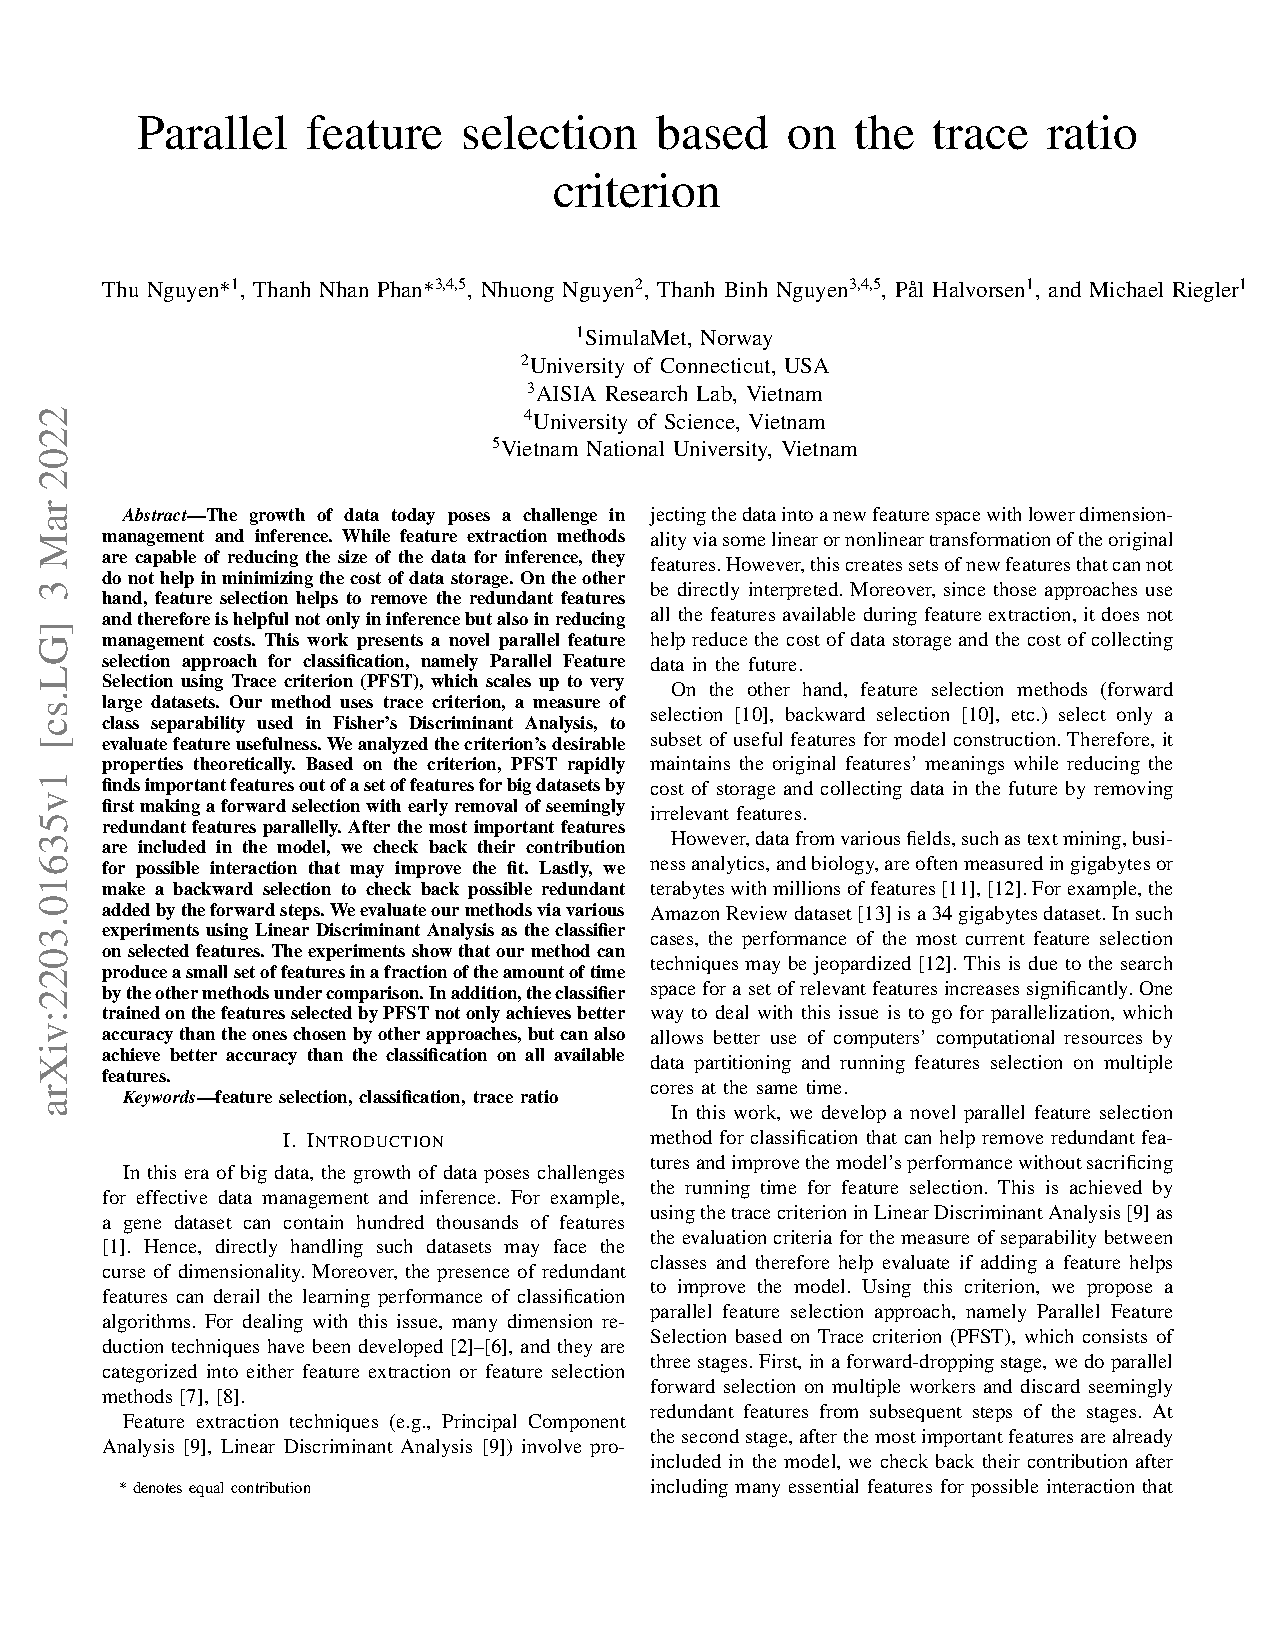
\includepdf[pages=-,scale=1]{2203.01635.pdf}
\lfoot{}
\cfoot{\thepage}
\rfoot{}

%\thispagestyle{empty}
\restoregeometry
	\newpage
	\addcontentsline{toc}{chapter}{\indexname}
	\printindex

\end{document}